    % Each problem--solution pair below is a self-contained movable unit.
    % To add, delete, or reorder problems, move the complete pair within its
    % category; numbering restarts from 1 in each category automatically.
    \expectedproblemsection{Standard Mathematical Problems}

    \begin{expectedproblem}[1988 IMO, Vieta Jumping]
        Let $a$ and $b$ be positive integers such that $ab+1$ divides
        $a^2+b^2$. Show that
        \[
            \frac{a^2+b^2}{ab+1}
        \]
        is the square of an integer.
    \end{expectedproblem}

    \begin{solution}
        Let
        \[
            k=\frac{a^2+b^2}{ab+1}\in\N.
        \]
        Suppose, for contradiction, that $k$ is not a perfect square. Among all
        positive integer solutions of
        \[
            a^2+b^2=k(ab+1),
        \]
        choose one for which $a+b$ is minimal, and assume without loss of
        generality that $a\geq b$.

        If $a=b$, then
        \[
            k=\frac{2a^2}{a^2+1}<2,
        \]
        so $k=1$, a contradiction. Hence $a>b$. Regard the equation as a
        quadratic equation in $a$:
        \[
            x^2-kbx+b^2-k=0.
        \]
        One root is $a$, so the other root is
        \[
            c=kb-a\in\Z.
        \]
        We claim that $c>0$. From
        \[
            a(a-kb)=k-b^2,
        \]
        if $a=kb$, then $k=b^2$, contrary to the assumption. If $a>kb$, then
        the left-hand side is at least $a\geq kb\geq k$, whereas the
        right-hand side is less than $k$, which is impossible. Therefore
        $a<kb$, and hence $c>0$.

        Since $k$ is a positive integer that is not a perfect square, we have
        $k\geq2$. Let
        \[
            f(x)=x^2-kbx+b^2-k.
        \]
        Since
        \[
            f(b)=(2-k)b^2-k<0
        \]
        and the two roots are $c$ and $a$ with $a>b$, it follows that
        \[
            0<c<b.
        \]
        By Vi\`ete's formulas, $c$ is the other root, and therefore
        \[
            c^2+b^2=k(cb+1).
        \]
        Thus $(c,b)$ is another positive integer solution with
        \[
            c+b<a+b,
        \]
        contradicting the minimality of $a+b$. Hence $k$ must be a perfect
        square.
    \end{solution}

    \begin{expectedproblem}[Sophomore's Dream]
        Prove the identity
        \[
            \int_0^1 x^{-x}\dd x
            =
            \sum_{n=1}^{\infty}\frac{1}{n^n}.
        \]
    \end{expectedproblem}

    \begin{solution}
        For $0<x\leq1$, we have $-\ln x\geq0$, and hence
        \[
            x^{-x}
            =
            e^{-x\ln x}
            =
            \sum_{n=0}^{\infty}
            \frac{x^n(-\ln x)^n}{n!}.
        \]
        Every term is nonnegative, so Tonelli's theorem from Mathematical
        Concepts permits term-by-term integration:
        \[
            \int_0^1x^{-x}\dd x
            =
            \sum_{n=0}^{\infty}
            \frac{1}{n!}
            \int_0^1x^n(-\ln x)^n\dd x.
        \]
        In the $n$th integral, let $t=-(n+1)\ln x$. Then
        \[
            \int_0^1x^n(-\ln x)^n\dd x
            =
            \frac{1}{(n+1)^{n+1}}
            \int_0^\infty t^ne^{-t}\dd t
            =
            \frac{n!}{(n+1)^{n+1}}.
        \]
        Therefore
        \[
            \int_0^1x^{-x}\dd x
            =
            \sum_{n=0}^{\infty}\frac{1}{(n+1)^{n+1}}
            =
            \boxed{\sum_{n=1}^{\infty}\frac{1}{n^n}}.
        \]
        Numerically, the common value is approximately
        \[
            1.291285997\ldots.
        \]
    \end{solution}

    \begin{expectedproblem}[1982 IMO]
        A function
        \[
            f:\Z_{>0}\to\Z_{\geq0}
        \]
        satisfies
        \[
            f(m+n)-f(m)-f(n)\in\{0,1\}
        \]
        for all positive integers $m$ and $n$. Moreover,
        \[
            f(2)=0,
            \qquad
            f(3)>0,
            \qquad
            f(9999)=3333.
        \]
        Determine $f(1982)$.
    \end{expectedproblem}

    \begin{solution}
        Repeatedly applying the given condition shows that, for all positive
        integers $r$ and $t$,
        \[
            r f(t)
            \leq
            f(rt)
            \leq
            r f(t)+r-1.
        \]
        Apply this estimate to
        \[
            N=9999\cdot1982
        \]
        in two different ways. Using $t=1982$ and then $t=9999$ gives
        \[
            9999f(1982)
            \leq
            f(N)
            \leq
            9999f(1982)+9998
        \]
        and
        \[
            1982\cdot3333
            \leq
            f(N)
            \leq
            1982\cdot3333+1981.
        \]
        Consequently,
        \[
            \frac{1982\cdot3333-9998}{9999}
            \leq
            f(1982)
            \leq
            \frac{1982\cdot3333+1981}{9999}.
        \]
        The left endpoint lies strictly between $659$ and $660$, whereas the
        right endpoint lies strictly between $660$ and $661$. Since
        $f(1982)$ is an integer, it follows that
        \[
            \boxed{f(1982)=660}.
        \]
    \end{solution}

    \begin{expectedproblem}[Happy Ending Problem]
        Five points are given in the plane, no three of which are collinear.
        Prove that four of them are the vertices of a convex quadrilateral.
    \end{expectedproblem}

    \begin{solution}
        Consider the convex hull of the five points. If the convex hull has at
        least four vertices, any four of its vertices, taken in cyclic order,
        form a convex quadrilateral.

        It remains to consider the case in which the convex hull is a triangle
        with vertices $A,B,C$. Let the remaining two points be $P$ and $Q$;
        both lie in the interior of $\triangle ABC$. The line $PQ$ contains none
        of $A,B,C$, so two of the three vertices lie in the same open half-plane
        determined by $PQ$. Relabel them as $A$ and $B$.

        The triangle $\triangle ABQ$ meets the line $PQ$ only at $Q$, because
        $A$ and $B$ lie strictly on the same side of that line. Hence
        $P\notin\triangle ABQ$. Similarly, $Q\notin\triangle ABP$. Since
        $A$ and $B$ are vertices of the convex hull of all five points, neither
        lies in the triangle determined by the other three points. Consequently,
        all four points $A,B,P,Q$ are vertices of their convex hull, which is a
        convex quadrilateral.
    \end{solution}

    \begin{expectedproblem}[Sylvester--Gallai Theorem]
        Let $S$ be a finite set of points in the plane, not all collinear. Prove
        that there exists a line containing exactly two points of $S$.
    \end{expectedproblem}

    \begin{solution}
        Call a line determined by points of $S$ \emph{ordinary} if it contains
        exactly two points of $S$. Consider all pairs $(P,\ell)$ such that
        $P\in S$, the line $\ell$ is determined by at least two points of $S$,
        and $P\notin\ell$. Since $S$ is finite and not collinear, the set of
        positive distances arising in this way is finite and nonempty. Choose
        $(P,\ell)$ so that
        \[
            h=\dist(P,\ell)>0
        \]
        is as small as possible, and let $H$ be the foot of the perpendicular
        from $P$ to $\ell$.

        Suppose, for contradiction, that $\ell$ contains at least three points
        of $S$. We can choose distinct points $A,B\in S\cap\ell$ so that either
        $A=H$, or $A$ and $B$ lie on the same side of $H$ with $A$ closer to
        $H$. In either case,
        \[
            AB<PB.
        \]
        Indeed, if $A=H$, then $AB=HB<PB$; otherwise,
        $AB=HB-HA<HB<PB$.

        Computing the area of $\triangle PAB$ with bases $AB$ and $PB$ gives
        \[
            \frac12 AB\,h
            =
            [PAB]
            =
            \frac12 PB\,\dist(A,PB).
        \]
        Hence
        \[
            \dist(A,PB)
            =
            \frac{AB}{PB}h
            <
            h.
        \]
        However, the line $PB$ is determined by two points of $S$, and
        $A\notin PB$. This contradicts the minimality of $h$.

        Therefore, $\ell$ contains exactly two points of $S$, so $\ell$ is the
        required ordinary line.
    \end{solution}

    \begin{expectedproblem}[Moser's Circle Problem]
        Let $n$ be a positive integer. Place $n$ points on a circle and join
        every pair of points by a chord.
        Assume that no three chords meet at a common point in the interior of
        the circle. Determine, with proof, the maximum number of regions into
        which the chords divide the circle.
    \end{expectedproblem}

    \begin{solution}
        There are
        \[
            \binom{n}{2}
        \]
        chords. Draw them one at a time. If a new chord contains $r$ existing
        interior intersection points, those points divide it into $r+1$
        segments, and each segment splits one existing region into two.
        Therefore the new chord creates $r+1$ new regions.

        It follows that the final number of regions is
        \[
            1
            +
            \#\{\text{chords}\}
            +
            \#\{\text{interior intersections}\}.
        \]
        Every interior intersection is determined by four boundary points:
        among the six chords joining those four points, exactly the two
        diagonals of their cyclic quadrilateral intersect in the interior.
        Conversely, every choice of four boundary points produces one such
        intersection. The assumption that no three chords are concurrent
        ensures that all these intersections are distinct. Hence there are
        \[
            \binom{n}{4}
        \]
        interior intersections.

        Thus the maximum number of regions is
        \[
            \boxed{
                1+\binom{n}{2}+\binom{n}{4}
            }.
        \]
        In particular, the first values are
        \[
            1,\ 2,\ 4,\ 8,\ 16,\ 31,\ldots,
        \]
        so the apparent pattern $2^{n-1}$ fails when $n=6$.
    \end{solution}

    \begin{expectedproblem}[1976 IMO]
        Determine, with proof, the largest number that can be written as the
        product of positive integers whose sum is $1976$. The number of
        factors is not prescribed.
    \end{expectedproblem}

    \begin{solution}
        A maximizing product contains no factor $1$, since replacing a pair
        $1,a$ by $a+1$ preserves the sum and increases the product. It also
        contains no factor $k\geq5$, because replacing $k$ by $3$ and $k-3$
        preserves the sum and increases the product:
        \[
            3(k-3)>k.
        \]
        A factor $4$ may be replaced by $2,2$ without changing the product.
        Thus it suffices to use only $2$ and $3$.

        Three factors equal to $2$ should be replaced by two factors equal to
        $3$, since
        \[
            2+2+2=3+3
            \qquad\text{and}\qquad
            2^3<3^2.
        \]
        Hence at most two factors equal to $2$ occur. Since
        \[
            1976=3\cdot658+2,
        \]
        the only optimal remainder pattern is one factor equal to $2$ and
        $658$ factors equal to $3$.

        Therefore, the largest possible product is
        \[
            \boxed{2\cdot3^{658}}.
        \]
    \end{solution}

    \begin{expectedproblem}[2021 Putnam]
        A grasshopper starts at the origin in the coordinate plane and makes a
        sequence of hops. Each hop has length $5$, and after every hop the
        grasshopper is at a point whose coordinates are both integers.
        Determine the smallest number of hops needed to reach
        \[
            (2021,2021).
        \]
    \end{expectedproblem}

    \begin{solution}
        If a hop has displacement vector $(p,q)$, then
        \[
            p^2+q^2=25.
        \]
        Thus the possible absolute coordinate pairs are $(5,0)$ and $(4,3)$,
        in either order. In particular, a single hop can increase the sum of
        the two coordinates by at most
        \[
            4+3=7.
        \]
        Since
        \[
            2021+2021=4042=7\cdot577+3,
        \]
        at least $578$ hops are necessary.

        This bound is attained because
        \[
            (2021,2021)
            =
            288(3,4)+288(4,3)+(5,0)+(0,5).
        \]
        The right-hand side is a sum of
        \[
            288+288+1+1=578
        \]
        legal hop vectors. Therefore, the minimum number of hops is
        \[
            \boxed{578}.
        \]
    \end{solution}

    \begin{expectedproblem}[Buffon's Needle]
        Infinitely many parallel lines are drawn in the plane, with distance
        $d$ between consecutive lines. A needle of length $\ell$, where
        \[
            0<\ell\leq d,
        \]
        is dropped at random. Assume that its midpoint is uniformly
        distributed modulo one strip and, independently, that its direction is
        uniformly distributed. Determine the probability that the needle
        intersects one of the parallel lines.
    \end{expectedproblem}

    \begin{solution}
        Let $X$ be the distance from the midpoint of the needle to the nearest
        parallel line, and let $\Theta$ be the acute angle between the needle
        and the lines. Then
        \[
            0\leq X\leq\frac{d}{2},
            \qquad
            0\leq\Theta\leq\frac{\pi}{2},
        \]
        and $X$ and $\Theta$ are independent and uniform on these intervals.

        For a fixed angle $\theta$, the needle intersects a line exactly when
        its perpendicular half-length reaches the nearest line, that is, when
        \[
            X\leq\frac{\ell}{2}\sin\theta.
        \]
        Since $\ell\leq d$, the right-hand side never exceeds $d/2$.
        Therefore,
        \[
            \begin{aligned}
                \Prob(\text{intersection})
                &=
                \frac{2}{\pi}
                \int_0^{\pi/2}
                \Prob\left(
                    X\leq\frac{\ell}{2}\sin\theta
                \right)\dd\theta\\
                &=
                \frac{2}{\pi}
                \int_0^{\pi/2}
                \frac{\ell\sin\theta}{d}\dd\theta\\
                &=
                \boxed{\frac{2\ell}{\pi d}}.
            \end{aligned}
        \]
    \end{solution}


    \begin{expectedproblem}[2011 IMO, Windmill Problem]
        Let $S$ be a finite set of at least two points in the plane, and assume
        that no three points of $S$ are collinear. A windmill is the following
        process. Start with a line $\ell$ through a point $P\in S$. Rotate
        $\ell$ clockwise about the pivot $P$ until it first meets another point
        $Q\in S$. The point $Q$ then becomes the new pivot, and the line
        continues to rotate clockwise. The process is repeated indefinitely.

        Prove that one can choose the initial point $P$ and the initial line
        $\ell$ so that every point of $S$ is used as a pivot infinitely many
        times.
    \end{expectedproblem}

    \begin{solution}
        Orient the rotating line and call its two open sides the left and right
        sides. When the pivot changes from $T$ to $U$, retain the orientation of
        the line. Immediately after the change, the old pivot $T$ lies on the
        same side on which $U$ lay immediately before the change. Hence the
        ordered numbers of points on the two sides are invariant throughout the
        process, except at the instants when the line contains two points of
        $S$.

        First suppose that
        \[
            |S|=2m+1.
        \]
        For every $T\in S$, there is an oriented line through $T$ with exactly
        $m$ points of $S$ on each side. To see this, rotate a line through $T$
        by an angle $\pi$. The number of points on its left changes by one at
        each encounter with another point of $S$, and its initial and final
        values sum to $2m$; therefore the value $m$ occurs.

        Choose such a balanced line through any point as the initial state. The
        side counts remain $(m,m)$. Fix $T\in S$ and choose a balanced line
        $r$ through $T$. Among all lines parallel to $r$, the line $r$ is the
        unique one that contains a point of $S$ and has $m$ points on each
        side: translating it in either direction changes the balance at the
        first point crossed. Consequently, when the windmill becomes parallel
        to $r$, it must coincide with $r$, so $T$ is a pivot. Thus every point
        is visited during each half-turn of the windmill line.

        Now suppose that
        \[
            |S|=2m.
        \]
        For every $T\in S$, the same half-turn argument gives an oriented line
        through $T$ with $m-1$ points on its left and $m$ points on its right.
        Start the windmill from one such line. Its ordered side counts remain
        $(m-1,m)$. For any prescribed $T$, choose an oriented line $r$ through
        $T$ with these counts. It is the unique oriented translate in its
        direction with these counts, so the windmill must pass through $T$ when
        it reaches that oriented direction. Hence every point is visited during
        each full turn.

        Only finitely many line directions are determined by pairs of points of
        $S$. Therefore the positive angular increments between successive pivot
        changes have a positive minimum. Since the process continues
        indefinitely, the total angle of rotation tends to infinity. The
        preceding half-turn or full-turn argument then applies repeatedly, and
        every point of $S$ is used as a pivot infinitely many times.
    \end{solution}

    \begin{expectedproblem}[Art Gallery Problem]
        A museum has the shape of a simple polygon with $n$ vertices. A guard
        must stand at a vertex of the polygon and can see a point whenever the
        entire line segment joining the guard to that point lies in the
        polygon. Prove that the entire museum can always be guarded by at most
        \[
            \left\lfloor\frac{n}{3}\right\rfloor
        \]
        guards.
    \end{expectedproblem}

    \begin{solution}
        Triangulate the polygon using nonintersecting diagonals between its
        vertices. The graph formed by the polygon sides and the triangulation
        diagonals admits a proper coloring with three colors.

        To prove this, use induction on $n$. The assertion is immediate for a
        triangle. Every triangulated polygon has an ear: a triangle in the
        triangulation with two sides on the boundary. Remove the ear vertex and
        color the remaining triangulated polygon by induction. The two
        neighbors of the removed vertex are adjacent and therefore have
        different colors, so the removed vertex can be assigned the third
        color. This completes the induction.

        Every triangle of the triangulation has one vertex of each color. Of
        the three color classes, one contains at most
        \[
            \left\lfloor\frac{n}{3}\right\rfloor
        \]
        vertices. Place guards at all vertices in that smallest color class.
        Every triangle contains one of these guards, and a guard at a vertex of
        a triangle sees every point of that triangle because a triangle is
        convex. Since the triangles cover the polygon, these guards see the
        entire museum.
    \end{solution}

    \begin{expectedproblem}[Bertrand's Ballot Problem]
        In an election, candidate $A$ receives $p$ votes and candidate $B$
        receives $q$ votes, where
        \[
            p>q.
        \]
        The $p+q$ ballots are counted in a uniformly random order. Determine
        the probability that, after every ballot is counted, the cumulative
        number of votes for $A$ is strictly greater than the cumulative number
        of votes for $B$.
    \end{expectedproblem}

    \begin{solution}
        Represent a vote for $A$ by a horizontal step and a vote for $B$ by a
        vertical step. A counting order is then a lattice path from $(0,0)$ to
        $(p,q)$, and the required condition is that the path remain strictly
        below the diagonal $y=x$ after leaving the origin.

        The first ballot must be for $A$. Remove this first horizontal step and
        translate the remaining path one unit to the left. We obtain a path
        from $(0,0)$ to $(p-1,q)$ that never enters the region $y>x$.
        By the reflection principle, the number of such paths is
        \[
            \binom{p+q-1}{q}
            -
            \binom{p+q-1}{q-1}.
        \]
        Since all
        \[
            \binom{p+q}{q}
        \]
        ballot orders are equally likely, the desired probability is
        \[
            \begin{aligned}
                \frac{
                    \binom{p+q-1}{q}-\binom{p+q-1}{q-1}
                }{
                    \binom{p+q}{q}
                }
                &=
                \frac{p-q}{p+q}.
            \end{aligned}
        \]
        Therefore the probability is
        \[
            \boxed{\frac{p-q}{p+q}}.
        \]
    \end{solution}

    \expectedproblemsection{Direct Calculation Problems}

    \begin{expectedproblem}[Finite Sums and Products]
        Evaluate each of the following finite sums or products exactly. State any
        restrictions on the integer parameters that are needed for the displayed
        expression to be defined.

        \begin{expectedsubproblem}[Vandermonde's Identity]
            For $n\in\Nzero$, determine
            \[
                \sum_{k=0}^{n}\binom{n}{k}^2.
            \]
        \end{expectedsubproblem}

        \begin{expectedsubproblem}
            For $n\in\Nzero$, determine
            \[
                \sum_{k=0}^{n}
                (-1)^k\binom{n}{k}\frac{1}{k+1}.
            \]
        \end{expectedsubproblem}

        \begin{expectedsubproblem}[Sine Product Formula]
            For an integer $n\geq2$, determine
            \[
                \prod_{k=1}^{n-1}\sin\left(\frac{k\pi}{n}\right).
            \]
        \end{expectedsubproblem}

        \begin{expectedsubproblem}
            For an integer $n\geq2$, determine
            \[
                \prod_{k=2}^{n}\frac{k^3-1}{k^3+1}.
            \]
        \end{expectedsubproblem}

        \begin{expectedsubproblem}[Double-Angle Product]
            For $m\in\N$ and $\sin x\neq0$, determine
            \[
                \prod_{k=0}^{m-1}\cos(2^k x).
            \]
        \end{expectedsubproblem}
    \end{expectedproblem}

    \begin{expectedsubsolution}
        Since
        \[
            \binom{n}{k}=\binom{n}{n-k},
        \]
        the required sum is the coefficient of $x^n$ in
        \[
            (1+x)^n(1+x)^n=(1+x)^{2n}.
        \]
        Therefore,
        \[
            \boxed{
                \sum_{k=0}^{n}\binom{n}{k}^2=\binom{2n}{n}
            }.
        \]
    \end{expectedsubsolution}

    \begin{expectedsubsolution}
        Using
        \[
            \frac{1}{k+1}=\int_0^1x^k\dd x,
        \]
        we obtain
        \[
            \begin{aligned}
                \sum_{k=0}^{n}
                (-1)^k\binom{n}{k}\frac{1}{k+1}
                &=
                \int_0^1
                \sum_{k=0}^{n}\binom{n}{k}(-x)^k\dd x\\
                &=
                \int_0^1(1-x)^n\dd x\\
                &=
                \boxed{\frac{1}{n+1}}.
            \end{aligned}
        \]
    \end{expectedsubsolution}

    \begin{expectedsubsolution}
        Let $\omega_n=e^{2\pi i/n}$. Factoring $z^n-1$ and then dividing by
        $z-1$ gives
        \[
            \frac{z^n-1}{z-1}
            =
            \prod_{k=1}^{n-1}(z-\omega_n^k).
        \]
        Letting $z\to1$ and taking absolute values yields
        \[
            n
            =
            \prod_{k=1}^{n-1}|1-\omega_n^k|
            =
            \prod_{k=1}^{n-1}
            2\sin\left(\frac{k\pi}{n}\right).
        \]
        Hence
        \[
            \boxed{
                \prod_{k=1}^{n-1}
                \sin\left(\frac{k\pi}{n}\right)
                =
                \frac{n}{2^{n-1}}
            }.
        \]
    \end{expectedsubsolution}

    \begin{expectedsubsolution}
        Factor each term as
        \[
            \frac{k^3-1}{k^3+1}
            =
            \frac{k-1}{k+1}
            \frac{k^2+k+1}{k^2-k+1}.
        \]
        The two products telescope separately:
        \[
            \prod_{k=2}^{n}\frac{k-1}{k+1}
            =
            \frac{2}{n(n+1)},
        \]
        and, since $k^2+k+1=(k+1)^2-(k+1)+1$,
        \[
            \prod_{k=2}^{n}
            \frac{k^2+k+1}{k^2-k+1}
            =
            \frac{n^2+n+1}{3}.
        \]
        Therefore,
        \[
            \boxed{
                \prod_{k=2}^{n}\frac{k^3-1}{k^3+1}
                =
                \frac{2(n^2+n+1)}{3n(n+1)}
            }.
        \]
    \end{expectedsubsolution}

    \begin{expectedsubsolution}
        Repeatedly apply
        \[
            \sin(2t)=2\sin t\cos t.
        \]
        This gives
        \[
            \sin(2^m x)
            =
            2^m\sin x
            \prod_{k=0}^{m-1}\cos(2^k x).
        \]
        Since $\sin x\neq0$,
        \[
            \boxed{
                \prod_{k=0}^{m-1}\cos(2^k x)
                =
                \frac{\sin(2^m x)}{2^m\sin x}
            }.
        \]
    \end{expectedsubsolution}

    \begin{expectedproblem}[Recurrence Relations]
        Determine the requested term, closed form, or residue for each of the
        following recursively defined sequences.

        \begin{expectedsubproblem}[2006 VTRMC]
            Let $F_0=0$, $F_1=1$, and
            \[
                F_{n+2}=F_{n+1}+F_n.
            \]
            Determine the last decimal digit of $F_{2006}$.
        \end{expectedsubproblem}

        \begin{expectedsubproblem}
            Let
            \[
                a_0=2,
                \qquad
                a_1=\sqrt2,
                \qquad
                a_{n+2}=\sqrt2\,a_{n+1}-a_n.
            \]
            Determine $a_{2026}$.
        \end{expectedsubproblem}

        \begin{expectedsubproblem}[Newton's Method]
            Let $a_0=1$ and
            \[
                a_{n+1}
                =
                \frac12\left(a_n+\frac{2}{a_n}\right).
            \]
            Determine a closed form for $a_n$.
        \end{expectedsubproblem}

        \begin{expectedsubproblem}
            Let
            \[
                a_0=2\cos\left(\frac{2\pi}{7}\right),
                \qquad
                a_{n+1}=a_n^2-2.
            \]
            Determine $a_{2026}$.
        \end{expectedsubproblem}

        \begin{expectedsubproblem}
            Let $a_0=0$ and
            \[
                a_{n+1}=\frac{1+a_n}{2+a_n}.
            \]
            Determine a closed form for $a_n$ in terms of the Fibonacci
            sequence.
        \end{expectedsubproblem}
    \end{expectedproblem}

    \begin{expectedsubsolution}
        Modulo $2$, the Fibonacci sequence has period $3$:
        \[
            0,1,1,0,1,1,\ldots.
        \]
        Hence
        \[
            F_{2006}\equiv F_2\equiv1\pmod2.
        \]
        Also
        \[
            F_{n+5}=5F_{n+1}+3F_n,
        \]
        so modulo $5$,
        \[
            F_{n+5}\equiv3F_n.
        \]
        Iterating four times gives $F_{n+20}\equiv F_n\pmod5$. Therefore
        \[
            F_{2006}\equiv F_6=8\equiv3\pmod5.
        \]
        The unique decimal digit that is odd and congruent to $3$ modulo $5$ is
        \[
            \boxed{3}.
        \]
    \end{expectedsubsolution}

    \begin{expectedsubsolution}
        The sequence
        \[
            b_n=2\cos\left(\frac{n\pi}{4}\right)
        \]
        has the same initial values and satisfies
        \[
            b_{n+2}
            =
            2\cos\left(\frac{\pi}{4}\right)b_{n+1}-b_n
            =
            \sqrt2\,b_{n+1}-b_n.
        \]
        Hence $a_n=b_n$. Since $2026\equiv2\pmod8$,
        \[
            \boxed{
                a_{2026}
                =
                2\cos\left(\frac{2026\pi}{4}\right)
                =0
            }.
        \]
    \end{expectedsubsolution}

    \begin{expectedsubsolution}
        Set
        \[
            r_n=\frac{a_n-\sqrt2}{a_n+\sqrt2}.
        \]
        Direct substitution into the recurrence gives
        \[
            r_{n+1}=r_n^2.
        \]
        Moreover,
        \[
            r_0
            =
            \frac{1-\sqrt2}{1+\sqrt2}
            =
            -(3-2\sqrt2).
        \]
        Thus
        \[
            r_n=\bigl(-(3-2\sqrt2)\bigr)^{2^n}.
        \]
        Solving the defining relation for $a_n$ yields
        \[
            \boxed{
                a_n
                =
                \sqrt2\,
                \frac{1+r_n}{1-r_n},
                \qquad
                r_n=\bigl(-(3-2\sqrt2)\bigr)^{2^n}
            }.
        \]
    \end{expectedsubsolution}

    \begin{expectedsubsolution}
        The double-angle identity gives
        \[
            (2\cos\theta)^2-2=2\cos(2\theta).
        \]
        Hence induction yields
        \[
            a_n
            =
            2\cos\left(\frac{2^{n+1}\pi}{7}\right).
        \]
        Powers of $2$ modulo $14$ have period $3$, and
        \[
            2^{2027}\equiv4\pmod{14}.
        \]
        Therefore,
        \[
            \boxed{
                a_{2026}=2\cos\left(\frac{4\pi}{7}\right)
            }.
        \]
    \end{expectedsubsolution}

    \begin{expectedsubsolution}
        Let $(F_n)$ be the Fibonacci sequence with $F_0=0$ and $F_1=1$. We
        claim that
        \[
            a_n=\frac{F_{2n}}{F_{2n+1}}.
        \]
        The formula holds for $n=0$. If it holds for $n$, then
        \[
            \begin{aligned}
                a_{n+1}
                &=
                \frac{F_{2n}+F_{2n+1}}
                {F_{2n}+2F_{2n+1}}\\
                &=
                \frac{F_{2n+2}}{F_{2n+3}}.
            \end{aligned}
        \]
        Thus
        \[
            \boxed{a_n=\frac{F_{2n}}{F_{2n+1}}}.
        \]
    \end{expectedsubsolution}

    \begin{expectedproblem}[Limits]
        Evaluate each of the following limits. In parameterized problems,
        determine the exact value for every parameter regime stated in the
        subproblem.

        \begin{expectedsubproblem}[2012 \KAIST{} Problem of the Week, A limit of a sequence involving a square root]
            Let $a_0=3$ and
            \[
                a_n=a_{n-1}+\sqrt{a_{n-1}^2+3},
                \qquad n\geq1.
            \]
            Determine
            \[
                \lim_{n\to\infty}\frac{a_n}{2^n}.
            \]
        \end{expectedsubproblem}

        \begin{expectedsubproblem}[2013 \KAIST{} Problem of the Week, Limit of a sequence]
            For $a,b\in\R$, determine
            \[
                \lim_{n\to\infty}
                n\left(
                    1-\frac{a}{n}-\frac{b\ln(n+1)}{n}
                \right)^n.
            \]
        \end{expectedsubproblem}

        \begin{expectedsubproblem}[2014 \KAIST{} Problem of the Week, Limit]
            For $x\geq0$, let
            \[
                f_n(x)
                =
                \frac{
                    \displaystyle\prod_{k=1}^{n-1}(x+k)(x+k+1)
                }{(n!)^2}.
            \]
            Determine
            \[
                \lim_{n\to\infty}f_n(x).
            \]
        \end{expectedsubproblem}

        \begin{expectedsubproblem}[2016 \KAIST{} Problem of the Week, Integral limit]
            For $a\geq0$, determine
            \[
                \lim_{n\to\infty}
                n\int_{-1}^{0}
                \left(x+\frac{x^2}{2}+e^{ax}\right)^n\dd x.
            \]
        \end{expectedsubproblem}

        \begin{expectedsubproblem}[2023 \KAIST{} Problem of the Week, A limit]
            Determine
            \[
                \lim_{n\to\infty}
                \left(
                    \frac{\displaystyle\sum_{k=1}^{n+2}k^k}
                    {\displaystyle\sum_{k=1}^{n+1}k^k}
                    -
                    \frac{\displaystyle\sum_{k=1}^{n+1}k^k}
                    {\displaystyle\sum_{k=1}^{n}k^k}
                \right).
            \]
        \end{expectedsubproblem}
    \end{expectedproblem}

    \begin{expectedsubsolution}
        Write
        \[
            a_n=\sqrt3\cot\theta_n.
        \]
        Since $a_0=3$, we may take $\theta_0=\pi/6$. The half-angle identity
        \[
            \cot\frac{\theta}{2}=\cot\theta+\csc\theta
        \]
        transforms the recurrence into
        \[
            a_n
            =
            \sqrt3\left(\cot\theta_{n-1}+\csc\theta_{n-1}\right)
            =
            \sqrt3\cot\frac{\theta_{n-1}}{2}.
        \]
        Hence
        \[
            \theta_n=\frac{\pi}{6\cdot2^n}
            \qquad\text{and}\qquad
            a_n=\sqrt3\cot\left(\frac{\pi}{6\cdot2^n}\right).
        \]
        Using $t\cot t\to1$ as $t\to0$, we obtain
        \[
            \boxed{
                \lim_{n\to\infty}\frac{a_n}{2^n}
                =
                \frac{6\sqrt3}{\pi}
            }.
        \]
    \end{expectedsubsolution}

    \begin{expectedsubsolution}
        Put
        \[
            c_n=a+b\ln(n+1).
        \]
        Since $c_n/n\to0$ and $c_n^2/n\to0$, the logarithmic expansion gives
        \[
            n\ln\left(1-\frac{c_n}{n}\right)
            =
            -c_n+o(1).
        \]
        Therefore,
        \[
            n\left(1-\frac{c_n}{n}\right)^n
            =
            e^{-a}n(n+1)^{-b}\bigl(1+o(1)\bigr).
        \]
        It follows that the limit is
        \[
            \boxed{
                \begin{cases}
                    \infty, & b<1,\\
                    e^{-a}, & b=1,\\
                    0, & b>1.
                \end{cases}
            }
        \]
    \end{expectedsubsolution}

    \begin{expectedsubsolution}
        The Gamma function gives
        \[
            f_n(x)
            =
            \frac{\Gamma(n+x)\Gamma(n+x+1)}
            {\Gamma(x+1)\Gamma(x+2)\Gamma(n+1)^2}.
        \]
        Using
        \[
            \frac{\Gamma(n+\alpha)}{\Gamma(n+\beta)}
            \sim n^{\alpha-\beta},
        \]
        we obtain
        \[
            f_n(x)
            \sim
            \frac{n^{2x-1}}{\Gamma(x+1)\Gamma(x+2)}.
        \]
        Consequently,
        \[
            \boxed{
                \lim_{n\to\infty}f_n(x)
                =
                \begin{cases}
                    0, & 0\leq x<\dfrac12,\\[4pt]
                    \dfrac{8}{3\pi}, & x=\dfrac12,\\[6pt]
                    \infty, & x>\dfrac12.
                \end{cases}
            }
        \]
    \end{expectedsubsolution}

    \begin{expectedsubsolution}
        Let
        \[
            g(x)=x+\frac{x^2}{2}+e^{ax}.
        \]
        On $[-1,0]$, we have $-1/2\leq g(x)\leq1$, with equality $g(x)=1$
        only at $x=0$. Moreover,
        \[
            g(0)=1
            \qquad\text{and}\qquad
            g'(0)=1+a.
        \]
        The contribution from every interval $[-1,-\delta]$ is exponentially
        small. On the remaining interval, set $x=-t/n$. For each fixed $t\geq0$,
        \[
            g\left(-\frac{t}{n}\right)^n
            \longrightarrow
            e^{-(1+a)t}.
        \]
        A uniform exponential bound near the endpoint permits dominated
        convergence, and therefore
        \[
            \begin{aligned}
                \lim_{n\to\infty}
                n\int_{-1}^{0}g(x)^n\dd x
                &=
                \int_0^\infty e^{-(1+a)t}\dd t\\
                &=
                \boxed{\frac{1}{1+a}}.
            \end{aligned}
        \]
    \end{expectedsubsolution}

    \begin{expectedsubsolution}
        Let
        \[
            S_n=\sum_{k=1}^{n}k^k.
        \]
        The final two terms dominate the sum:
        \[
            S_n
            =
            n^n\left(1+\frac{1}{en}+O\left(\frac{1}{n^2}\right)\right).
        \]
        Hence
        \[
            \begin{aligned}
                \frac{S_{n+1}}{S_n}
                &=
                (n+1)\left(1+\frac{1}{n}\right)^n
                \frac{
                    1+\dfrac{1}{e(n+1)}+O(n^{-2})
                }{
                    1+\dfrac{1}{en}+O(n^{-2})
                }\\
                &=
                en+\frac{e}{2}+O\left(\frac{1}{n}\right).
            \end{aligned}
        \]
        Replacing $n$ by $n+1$ and subtracting gives
        \[
            \boxed{
                \lim_{n\to\infty}
                \left(
                    \frac{S_{n+2}}{S_{n+1}}
                    -
                    \frac{S_{n+1}}{S_n}
                \right)
                =e
            }.
        \]
    \end{expectedsubsolution}

    \begin{expectedproblem}[Derivatives]
        Compute each requested derivative or derivative-dependent quantity
        exactly. For high-order derivatives, a closed form involving standard
        sequences or harmonic numbers is acceptable.

        \begin{expectedsubproblem}[2006 HMMT]
            A nonzero polynomial $f\in\R[x]$ satisfies
            \[
                f(x)=f'(x)f''(x).
            \]
            Determine the leading coefficient of $f$.
        \end{expectedsubproblem}

        \begin{expectedsubproblem}[1993 VTRMC]
            For $x>0$, define
            \[
                f_1(x)=x,
                \qquad
                f_{n+1}(x)=x^{f_n(x)}.
            \]
            Determine $f_{2026}''(1)$.
        \end{expectedsubproblem}

        \begin{expectedsubproblem}
            Let
            \[
                f(x)=\frac{1}{1-x-x^2}.
            \]
            Determine $f^{(2026)}(0)$ in terms of the Fibonacci sequence.
        \end{expectedsubproblem}

        \begin{expectedsubproblem}
            Determine
            \[
                \left.
                \frac{\dd^{2026}}{\dd x^{2026}}
                \bigl(e^x\sin x\bigr)
                \right|_{x=0}.
            \]
        \end{expectedsubproblem}

        \begin{expectedsubproblem}[Leibniz's Rule]
            Let
            \[
                H_n=\sum_{k=1}^{n}\frac{1}{k}.
            \]
            Determine
            \[
                \left.
                \frac{\dd^{100}}{\dd x^{100}}
                \bigl(x^{100}\ln x\bigr)
                \right|_{x=1}.
            \]
        \end{expectedsubproblem}
    \end{expectedproblem}

    \begin{expectedsubsolution}
        Suppose that the leading term of $f$ is $cx^n$, where $c\neq0$. The
        leading term of $f'f''$ is
        \[
            c^2n^2(n-1)x^{2n-3}.
        \]
        Comparing degrees gives
        \[
            n=2n-3,
        \]
        so $n=3$. Comparing leading coefficients then gives
        \[
            c=18c^2.
        \]
        Since $c\neq0$,
        \[
            \boxed{c=\frac{1}{18}}.
        \]
    \end{expectedsubsolution}

    \begin{expectedsubsolution}
        Since $f_n(1)=1$ for every $n$, take logarithms:
        \[
            \ln f_{n+1}(x)=f_n(x)\ln x.
        \]
        Differentiating and evaluating at $x=1$ shows inductively that
        \[
            f_n'(1)=1.
        \]
        Put $g(x)=\ln f_{n+1}(x)$. Then
        \[
            g'(1)=1
            \qquad\text{and}\qquad
            g''(1)=2f_n'(1)-f_n(1)=1.
        \]
        Since $f_{n+1}=e^g$,
        \[
            f_{n+1}''(1)
            =
            f_{n+1}(1)\bigl(g'(1)^2+g''(1)\bigr)
            =2.
        \]
        Therefore,
        \[
            \boxed{f_{2026}''(1)=2}.
        \]
    \end{expectedsubsolution}

    \begin{expectedsubsolution}
        The ordinary generating function of the Fibonacci sequence is
        \[
            \frac{1}{1-x-x^2}
            =
            \sum_{n=0}^{\infty}F_{n+1}x^n,
        \]
        where $F_0=0$ and $F_1=1$. Therefore the coefficient of $x^{2026}$ is
        $F_{2027}$, and
        \[
            \boxed{f^{(2026)}(0)=2026!\,F_{2027}}.
        \]
    \end{expectedsubsolution}

    \begin{expectedsubsolution}
        Since
        \[
            e^x\sin x
            =
            \Imag\bigl(e^{(1+i)x}\bigr),
        \]
        the required derivative is
        \[
            \Imag\bigl((1+i)^{2026}\bigr).
        \]
        Now
        \[
            (1+i)^{2026}
            =
            2^{1013}e^{i2026\pi/4}
            =
            2^{1013}i.
        \]
        Hence the value is
        \[
            \boxed{2^{1013}}.
        \]
    \end{expectedsubsolution}

    \begin{expectedsubsolution}
        For a real parameter $\alpha$,
        \[
            \frac{\dd^{100}}{\dd x^{100}}x^\alpha
            =
            \alpha(\alpha-1)\cdots(\alpha-99)x^{\alpha-100}.
        \]
        Differentiate both sides with respect to $\alpha$ and then set
        $\alpha=100$ and $x=1$. Since
        \[
            \left.
            \frac{\dd}{\dd\alpha}
            \prod_{j=0}^{99}(\alpha-j)
            \right|_{\alpha=100}
            =
            100!\sum_{k=1}^{100}\frac{1}{k},
        \]
        we obtain
        \[
            \boxed{100!\,H_{100}}.
        \]
    \end{expectedsubsolution}

    \begin{expectedproblem}[Series]
        Determine whether each of the following series converges. For every
        convergent series, determine its exact sum. In parameterized problems,
        state all parameter values for which convergence occurs.

        \begin{expectedsubproblem}[2016 \KAIST{} Problem of the Week, A series]
            Let $k$ be a positive integer, and define
            \[
                a_n
                =
                \begin{cases}
                    1, & (k+1)\nmid n,\\
                    -k, & (k+1)\mid n.
                \end{cases}
            \]
            Determine
            \[
                \sum_{n=1}^{\infty}\frac{a_n}{n}.
            \]
        \end{expectedsubproblem}

        \begin{expectedsubproblem}[2017 \KAIST{} Problem of the Week, Convergence of a series]
            Determine whether
            \[
                \sum_{n=0}^{\infty}
                \frac{1}{4^n}\binom{2n}{n}
            \]
            converges.
        \end{expectedsubproblem}

        \begin{expectedsubproblem}[2011 \KAIST{} Problem of the Week, A Series]
            Determine
            \[
                \sum_{n=1}^{\infty}\frac{n\sin n}{1+n^2}.
            \]
        \end{expectedsubproblem}

        \begin{expectedsubproblem}[2014 \KAIST{} Problem of the Week, Series]
            Determine all positive integers $\ell$ for which
            \[
                \sum_{n=1}^{\infty}
                \frac{n^3}{(n+1)(n+2)\cdots(n+\ell)}
            \]
            converges, and compute its value whenever it converges.
        \end{expectedsubproblem}

        \begin{expectedsubproblem}[2024 \KAIST{} Problem of the Week, Infinite series of reciprocals]
            Determine
            \[
                \sum_{k=0}^{\infty}
                \frac{1}{
                    (6k+1)(6k+2)(6k+3)(6k+4)(6k+5)(6k+6)
                }.
            \]
        \end{expectedsubproblem}
    \end{expectedproblem}

    \begin{expectedsubsolution}
        At the end of the $N$th complete block of length $k+1$, the partial sum
        is
        \[
            \begin{aligned}
                \sum_{n=1}^{(k+1)N}\frac{a_n}{n}
                &=
                \sum_{n=1}^{(k+1)N}\frac{1}{n}
                -(k+1)\sum_{m=1}^{N}\frac{1}{(k+1)m}\\
                &=
                H_{(k+1)N}-H_N.
            \end{aligned}
        \]
        Since $H_N=\ln N+\gamma+o(1)$, these partial sums tend to
        $\ln(k+1)$. The terms inside the final incomplete block tend uniformly
        to zero, so the full series has the same limit. Therefore,
        \[
            \boxed{
                \sum_{n=1}^{\infty}\frac{a_n}{n}=\ln(k+1)
            }.
        \]
    \end{expectedsubsolution}

    \begin{expectedsubsolution}
        By the central binomial coefficient asymptotic,
        \[
            \frac{1}{4^n}\binom{2n}{n}
            \sim
            \frac{1}{\sqrt{\pi n}}.
        \]
        Since the $p$-series $\sum n^{-1/2}$ diverges, the limit comparison
        test gives
        \[
            \boxed{
                \sum_{n=0}^{\infty}
                \frac{1}{4^n}\binom{2n}{n}
                \text{ diverges}
            }.
        \]
    \end{expectedsubsolution}

    \begin{expectedsubsolution}
        For $a>0$ and $0<x<2\pi$, the standard Fourier expansion is
        \[
            \sum_{n=-\infty}^{\infty}
            \frac{e^{inx}}{n^2+a^2}
            =
            \frac{\pi}{a}
            \frac{\cosh(a(\pi-x))}{\sinh(a\pi)}.
        \]
        Differentiating with respect to $x$ and comparing real quantities gives
        \[
            \sum_{n=1}^{\infty}
            \frac{n\sin(nx)}{n^2+a^2}
            =
            \frac{\pi}{2}
            \frac{\sinh(a(\pi-x))}{\sinh(a\pi)}.
        \]
        Setting $a=1$ and $x=1$, we obtain
        \[
            \boxed{
                \sum_{n=1}^{\infty}\frac{n\sin n}{1+n^2}
                =
                \frac{\pi}{2}
                \frac{\sinh(\pi-1)}{\sinh\pi}
            }.
        \]
    \end{expectedsubsolution}

    \begin{expectedsubsolution}
        The $n$th term is asymptotic to $n^{3-\ell}$, so the series converges
        exactly when
        \[
            \ell\geq5.
        \]
        For such $\ell$, the beta-integral identity gives
        \[
            \frac{1}{(n+1)(n+2)\cdots(n+\ell)}
            =
            \frac{1}{(\ell-1)!}
            \int_0^1x^n(1-x)^{\ell-1}\dd x.
        \]
        Since
        \[
            \sum_{n=1}^{\infty}n^3x^n
            =
            \frac{x(1+4x+x^2)}{(1-x)^4},
        \]
        term-by-term integration yields
        \[
            \begin{aligned}
                \sum_{n=1}^{\infty}
                \frac{n^3}{(n+1)\cdots(n+\ell)}
                &=
                \frac{1}{(\ell-1)!}
                \int_0^1x(1+4x+x^2)(1-x)^{\ell-5}\dd x\\
                &=
                \boxed{
                    \frac{\ell(\ell+5)}{
                        (\ell-4)(\ell-3)(\ell-2)(\ell-1)(\ell-1)!
                    }
                }.
            \end{aligned}
        \]
    \end{expectedsubsolution}

    \begin{expectedsubsolution}
        The beta-integral identity gives
        \[
            \frac{1}{(6k+1)(6k+2)\cdots(6k+6)}
            =
            \frac{1}{5!}\int_0^1x^{6k}(1-x)^5\dd x.
        \]
        Hence
        \[
            S
            =
            \frac{1}{120}
            \int_0^1\frac{(1-x)^5}{1-x^6}\dd x.
        \]
        The rational function decomposes as
        \[
            \frac{(1-x)^5}{1-x^6}
            =
            -\frac{9(x+1)}{2(x^2+x+1)}
            +
            \frac{x+1}{6(x^2-x+1)}
            +
            \frac{16}{3(x+1)}.
        \]
        Direct integration on $[0,1]$ therefore gives
        \[
            \boxed{
                S
                =
                \frac{2}{45}\ln2
                -\frac{3}{160}\ln3
                -\frac{7\sqrt3\pi}{4320}
            }.
        \]
    \end{expectedsubsolution}

    \begin{expectedproblem}[Integrals]
        Evaluate each of the following integrals. For indefinite integrals, the
        constant of integration may be omitted; for definite integrals,
        determine the exact value.

        \begin{expectedsubproblem}[2010 \MIT{} Integration Bee]
            \(\displaystyle
                \int_0^{\pi/2}\sin x\sin(2x)\sin(3x)\dd x
            \)
        \end{expectedsubproblem}

        \begin{expectedsubproblem}[2010 \MIT{} Integration Bee]
            \(\displaystyle
                \int_0^1\sin^2(\ln x)\dd x
            \)
        \end{expectedsubproblem}

        \begin{expectedsubproblem}[2010 \MIT{} Integration Bee]
            \(\displaystyle
                \int_1^\infty\frac{\dd x}{x\sqrt{x^4-1}}
            \)
        \end{expectedsubproblem}

        \begin{expectedsubproblem}[2010 \MIT{} Integration Bee]
            \(\displaystyle
                \int_0^1\frac{\ln(1+x)}{1+x^2}\dd x
            \)
        \end{expectedsubproblem}

        \begin{expectedsubproblem}[2010 \MIT{} Integration Bee]
            \(\displaystyle
                \int\frac{\cos x+x\sin x}{x(x+\cos x)}\dd x
            \)
        \end{expectedsubproblem}

        \begin{expectedsubproblem}[2010 \MIT{} Integration Bee]
            \(\displaystyle
                \int_0^{\pi/2}\frac{\dd x}{\sin x+\sec x}
            \)
        \end{expectedsubproblem}

        \begin{expectedsubproblem}[2010 \MIT{} Integration Bee]
            \(\displaystyle
                \int_0^1\sqrt{1+x\sqrt{1+x\sqrt{1+\cdots}}}\dd x
            \)
        \end{expectedsubproblem}

        \begin{expectedsubproblem}[2010 \MIT{} Integration Bee]
            \(\displaystyle
                \int\left(\frac{1}{\ln x}-\frac{1}{(\ln x)^2}\right)\dd x,
                \qquad x>0,\quad x\neq1
            \)
        \end{expectedsubproblem}

        \begin{expectedsubproblem}[2010 \MIT{} Integration Bee]
            \(\displaystyle
                \int_1^2\sqrt{x-1}\sqrt{2-x}\dd x
            \)
        \end{expectedsubproblem}

        \begin{expectedsubproblem}[2011 \MIT{} Integration Bee]
            \(\displaystyle
                \int\cos(\ln x)\dd x,
                \qquad x>0
            \)
        \end{expectedsubproblem}

        \begin{expectedsubproblem}[2011 \MIT{} Integration Bee]
            \(\displaystyle
                \int_0^\pi\cos x\cos(3x)\cos(5x)\dd x
            \)
        \end{expectedsubproblem}

        \begin{expectedsubproblem}[2011 \MIT{} Integration Bee]
            \(\displaystyle
                \int\sin(101x)\sin^{99}x\dd x
            \)
        \end{expectedsubproblem}

        \begin{expectedsubproblem}[2011 \MIT{} Integration Bee]
            \(\displaystyle
                \int x e^{e^{x^2}+x^2}\dd x
            \)
        \end{expectedsubproblem}

        \begin{expectedsubproblem}[2011 \MIT{} Integration Bee]
            \(\displaystyle
                \int\sqrt{\frac{1-x}{1+x}}\dd x,
                \qquad -1<x<1
            \)
        \end{expectedsubproblem}
    \end{expectedproblem}

    \begin{expectedsubsolution}
        By the product-to-sum identities,
        \[
            \sin x\sin(3x)
            =
            \frac{1}{2}\bigl(\cos(2x)-\cos(4x)\bigr),
        \]
        and hence
        \[
            \sin x\sin(2x)\sin(3x)
            =
            \frac{1}{4}
            \bigl(\sin(2x)+\sin(4x)-\sin(6x)\bigr).
        \]
        Therefore,
        \[
            \int_0^{\pi/2}\sin x\sin(2x)\sin(3x)\dd x
            =
            \frac{1}{4}\left(1-\frac{1}{3}\right)
            =
            \boxed{\frac{1}{6}}.
        \]
    \end{expectedsubsolution}

    \begin{expectedsubsolution}
        Let $t=-\ln x$. Then $x=e^{-t}$ and
        $\dd x=-e^{-t}\dd t$, so
        \[
            \int_0^1\sin^2(\ln x)\dd x
            =
            \int_0^\infty e^{-t}\sin^2t\dd t.
        \]
        Since $\sin^2t=(1-\cos(2t))/2$,
        \[
            \int_0^\infty e^{-t}\sin^2t\dd t
            =
            \frac{1}{2}
            \left(1-\frac{1}{5}\right)
            =
            \boxed{\frac{2}{5}}.
        \]
    \end{expectedsubsolution}

    \begin{expectedsubsolution}
        Let $u=x^2$. Then
        \[
            \frac{\dd x}{x}=\frac{\dd u}{2u},
        \]
        and therefore
        \[
            \int_1^\infty\frac{\dd x}{x\sqrt{x^4-1}}
            =
            \frac{1}{2}
            \int_1^\infty\frac{\dd u}{u\sqrt{u^2-1}}.
        \]
        With $u=\sec\theta$, this becomes
        \[
            \frac{1}{2}\int_0^{\pi/2}\dd\theta
            =
            \boxed{\frac{\pi}{4}}.
        \]
    \end{expectedsubsolution}

    \begin{expectedsubsolution}
        Let
        \[
            I=\int_0^1\frac{\ln(1+x)}{1+x^2}\dd x.
        \]
        Substituting $x=\tan t$ gives
        \[
            I=\int_0^{\pi/4}\ln(1+\tan t)\dd t.
        \]
        Under $t\mapsto\pi/4-t$,
        \[
            1+\tan\left(\frac{\pi}{4}-t\right)
            =
            \frac{2}{1+\tan t}.
        \]
        Thus
        \[
            I=\frac{\pi}{4}\ln2-I,
        \]
        and consequently
        \[
            \boxed{I=\frac{\pi}{8}\ln2}.
        \]
    \end{expectedsubsolution}

    \begin{expectedsubsolution}
        We recognize the logarithmic derivative
        \[
            \diff{}{x}
            \bigl(\ln|x|-\ln|x+\cos x|\bigr)
            =
            \frac{\cos x+x\sin x}{x(x+\cos x)}.
        \]
        Hence
        \[
            \boxed{
                \int\frac{\cos x+x\sin x}{x(x+\cos x)}\dd x
                =
                \ln|x|-\ln|x+\cos x|
            }.
        \]
    \end{expectedsubsolution}

    \begin{expectedsubsolution}
        Write
        \[
            I
            =
            \int_0^{\pi/2}
            \frac{\cos x}{1+\sin x\cos x}\dd x.
        \]
        Replacing $x$ by $\pi/2-x$ also gives
        \[
            I
            =
            \int_0^{\pi/2}
            \frac{\sin x}{1+\sin x\cos x}\dd x.
        \]
        Adding the two expressions and setting
        $u=\sin x-\cos x$, we obtain
        \[
            2I
            =
            \int_{-1}^{1}\frac{2}{3-u^2}\dd u.
        \]
        Therefore,
        \[
            \boxed{
                I=\frac{1}{\sqrt3}\ln(2+\sqrt3)
            }.
        \]
    \end{expectedsubsolution}

    \begin{expectedsubsolution}
        For $x\in[0,1]$, define the finite truncations by
        \[
            R_1(x)=1,
            \qquad
            R_{n+1}(x)=\sqrt{1+xR_n(x)}.
        \]
        Since $y\mapsto\sqrt{1+xy}$ is increasing for $x\in[0,1]$, induction
        gives
        \[
            1\leq R_n(x)\leq\varphi
            \qquad\text{and}\qquad
            R_n(x)\leq R_{n+1}(x),
        \]
        where $\varphi=(1+\sqrt5)/2$ and $\varphi^2=1+\varphi$. Hence
        $R_n(x)$ converges pointwise to a limit $R(x)$. Passing to the limit in
        the recurrence gives
        \[
            R(x)^2=1+xR(x),
        \]
        so positivity yields
        \[
            R(x)=\frac{x+\sqrt{x^2+4}}{2}.
        \]
        The uniform bound $0\leq R_n(x)\leq\varphi$ permits integration by the
        dominated convergence theorem. Therefore,
        \[
            \begin{aligned}
                \int_0^1R(x)\dd x
                &=
                \frac12\int_0^1x\dd x
                +
                \frac12\int_0^1\sqrt{x^2+4}\dd x\\
                &=
                \boxed{
                    \frac{1+\sqrt5}{4}
                    +
                    \ln\left(\frac{1+\sqrt5}{2}\right)
                }.
            \end{aligned}
        \]
    \end{expectedsubsolution}

    \begin{expectedsubsolution}
        On any interval contained in $(0,\infty)\setminus\{1\}$,
        \[
            \diff{}{x}\left(\frac{x}{\ln x}\right)
            =
            \frac{1}{\ln x}
            -
            \frac{1}{(\ln x)^2}.
        \]
        Therefore,
        \[
            \boxed{
                \int
                \left(
                    \frac{1}{\ln x}
                    -
                    \frac{1}{(\ln x)^2}
                \right)\dd x
                =
                \frac{x}{\ln x}
            }.
        \]
    \end{expectedsubsolution}

    \begin{expectedsubsolution}
        Let $u=x-1$. Then
        \[
            \int_1^2\sqrt{x-1}\sqrt{2-x}\dd x
            =
            \int_0^1\sqrt{u(1-u)}\dd u.
        \]
        Setting $v=u-1/2$ gives
        \[
            \sqrt{u(1-u)}
            =
            \sqrt{\frac{1}{4}-v^2}.
        \]
        Thus the integral is the area of a semicircle of radius $1/2$:
        \[
            \boxed{\frac{\pi}{8}}.
        \]
    \end{expectedsubsolution}

    \begin{expectedsubsolution}
        Let $t=\ln x$. Then $x=e^t$ and $\dd x=e^t\dd t$, so
        \[
            \int\cos(\ln x)\dd x
            =
            \int e^t\cos t\dd t.
        \]
        Therefore,
        \[
            \boxed{
                \int\cos(\ln x)\dd x
                =
                \frac{x}{2}
                \bigl(\cos(\ln x)+\sin(\ln x)\bigr)
            }.
        \]
    \end{expectedsubsolution}

    \begin{expectedsubsolution}
        By repeated use of the product-to-sum identity,
        \[
            \cos x\cos(3x)\cos(5x)
            =
            \frac{1}{4}
            \bigl(
                \cos x+\cos(3x)+\cos(7x)+\cos(9x)
            \bigr).
        \]
        Each term has integral $0$ on $[0,\pi]$. Hence
        \[
            \boxed{
                \int_0^\pi\cos x\cos(3x)\cos(5x)\dd x=0
            }.
        \]
    \end{expectedsubsolution}

    \begin{expectedsubsolution}
        Differentiating a suitable product gives
        \[
            \begin{aligned}
                \diff{}{x}
                \left(
                    \frac{1}{100}\sin(100x)\sin^{100}x
                \right)
                &=
                \sin^{99}x
                \bigl(
                    \sin x\cos(100x)
                    +
                    \cos x\sin(100x)
                \bigr)\\
                &=
                \sin(101x)\sin^{99}x.
            \end{aligned}
        \]
        Therefore,
        \[
            \boxed{
                \int\sin(101x)\sin^{99}x\dd x
                =
                \frac{1}{100}\sin(100x)\sin^{100}x
            }.
        \]
    \end{expectedsubsolution}

    \begin{expectedsubsolution}
        Since
        \[
            e^{e^{x^2}+x^2}=e^{e^{x^2}}e^{x^2},
        \]
        let $u=e^{x^2}$. Then $\dd u=2xe^{x^2}\dd x$, and
        \[
            \int x e^{e^{x^2}+x^2}\dd x
            =
            \frac{1}{2}\int e^u\dd u.
        \]
        Hence
        \[
            \boxed{
                \int x e^{e^{x^2}+x^2}\dd x
                =
                \frac{1}{2}e^{e^{x^2}}
            }.
        \]
    \end{expectedsubsolution}

    \begin{expectedsubsolution}
        For $-1<x<1$,
        \[
            \sqrt{\frac{1-x}{1+x}}
            =
            \frac{1-x}{\sqrt{1-x^2}}.
        \]
        Therefore,
        \[
            \begin{aligned}
                \int\sqrt{\frac{1-x}{1+x}}\dd x
                &=
                \int\frac{\dd x}{\sqrt{1-x^2}}
                -
                \int\frac{x}{\sqrt{1-x^2}}\dd x\\
                &=
                \boxed{\arcsin x+\sqrt{1-x^2}}.
            \end{aligned}
        \]
    \end{expectedsubsolution}

    \begin{expectedproblem}[Complex Numbers]
        Evaluate each of the following expressions exactly. When roots of unity
        occur, use $\omega_n=e^{2\pi i/n}$ unless another root is specified.

        \begin{expectedsubproblem}[De Moivre's Theorem]
            Determine $(1+i)^{2026}$.
        \end{expectedsubproblem}

        \begin{expectedsubproblem}
            Let $z\in\C\setminus\{0\}$ satisfy
            \[
                z+\frac{1}{z}=1.
            \]
            Determine
            \[
                z^{2026}+\frac{1}{z^{2026}}.
            \]
        \end{expectedsubproblem}

        \begin{expectedsubproblem}[Roots-of-Unity Filter]
            For an integer $n\geq2$, determine
            \[
                \sum_{k=0}^{n-1}(1+\omega_n^k)^n.
            \]
        \end{expectedsubproblem}

        \begin{expectedsubproblem}[Quadratic Gauss Sum]
            Let $\omega=e^{2\pi i/5}$. Determine
            \[
                \sum_{k=0}^{4}\omega^{k^2}.
            \]
        \end{expectedsubproblem}

        \begin{expectedsubproblem}
            For an integer $n\geq2$, determine
            \[
                \sum_{k=0}^{n-1}\frac{1}{2-\omega_n^k}.
            \]
        \end{expectedsubproblem}
    \end{expectedproblem}

    \begin{expectedsubsolution}
        Using polar form,
        \[
            1+i=\sqrt2\,e^{i\pi/4}.
        \]
        Hence
        \[
            (1+i)^{2026}
            =
            2^{1013}e^{i2026\pi/4}
            =
            \boxed{2^{1013}i}.
        \]
    \end{expectedsubsolution}

    \begin{expectedsubsolution}
        The equation is equivalent to
        \[
            z^2-z+1=0.
        \]
        Thus $z=e^{\pm i\pi/3}$, and therefore
        \[
            z^m+z^{-m}=2\cos\left(\frac{m\pi}{3}\right).
        \]
        Since $2026\equiv4\pmod6$,
        \[
            \boxed{
                z^{2026}+z^{-2026}
                =
                2\cos\left(\frac{4\pi}{3}\right)
                =-1
            }.
        \]
    \end{expectedsubsolution}

    \begin{expectedsubsolution}
        Expand by the binomial theorem and interchange the finite sums:
        \[
            \sum_{k=0}^{n-1}(1+\omega_n^k)^n
            =
            \sum_{j=0}^{n}\binom{n}{j}
            \sum_{k=0}^{n-1}\omega_n^{kj}.
        \]
        The inner sum is $n$ when $n\mid j$ and $0$ otherwise. For
        $0\leq j\leq n$, only $j=0$ and $j=n$ contribute. Hence
        \[
            \boxed{
                \sum_{k=0}^{n-1}(1+\omega_n^k)^n=2n
            }.
        \]
    \end{expectedsubsolution}

    \begin{expectedsubsolution}
        The quadratic residues modulo $5$ are
        \[
            0,1,4,4,1.
        \]
        Therefore,
        \[
            \sum_{k=0}^{4}\omega^{k^2}
            =
            1+2(\omega+\omega^{-1})
            =
            1+4\cos\left(\frac{2\pi}{5}\right).
        \]
        Since
        \[
            2\cos\left(\frac{2\pi}{5}\right)
            =
            \frac{\sqrt5-1}{2},
        \]
        the sum is
        \[
            \boxed{\sqrt5}.
        \]
    \end{expectedsubsolution}

    \begin{expectedsubsolution}
        Let
        \[
            p(z)=z^n-1
            =
            \prod_{k=0}^{n-1}(z-\omega_n^k).
        \]
        Its logarithmic derivative is
        \[
            \frac{p'(z)}{p(z)}
            =
            \sum_{k=0}^{n-1}\frac{1}{z-\omega_n^k}.
        \]
        Setting $z=2$ gives
        \[
            \boxed{
                \sum_{k=0}^{n-1}\frac{1}{2-\omega_n^k}
                =
                \frac{n2^{n-1}}{2^n-1}
            }.
        \]
    \end{expectedsubsolution}

    \begin{expectedproblem}[Polynomials and Roots]
        Use the coefficients, factorization, or symmetric functions of the roots
        to compute each requested quantity exactly. Solving every polynomial
        explicitly is not required unless the problem asks for the roots.

        \begin{expectedsubproblem}[2006 HMMT]
            Determine the sum of the distinct real roots of
            \[
                2x^6-3x^5+3x^4+x^3-3x^2+3x-1=0.
            \]
        \end{expectedsubproblem}

        \begin{expectedsubproblem}[1997 VTRMC]
            Two roots $r_1,r_2$ of
            \[
                x^4-x^3+ax^2-8x-8=0
            \]
            satisfy $r_1r_2=2$. Determine $a$, $r_1$, and $r_2$.
        \end{expectedsubproblem}

        \begin{expectedsubproblem}[Newton Sums]
            Let $\alpha_1,\ldots,\alpha_5$ be the roots of
            \[
                x^5-5x+3=0.
            \]
            Determine
            \[
                \sum_{j=1}^{5}
                \left(\alpha_j^4+\alpha_j^5\right).
            \]
        \end{expectedsubproblem}

        \begin{expectedsubproblem}[Logarithmic Derivative]
            Let $\alpha_1,\ldots,\alpha_4$ be the roots of
            \[
                x^4+x^3+x^2+x+1=0.
            \]
            Determine
            \[
                \sum_{j=1}^{4}\frac{1}{(1-\alpha_j)^2}.
            \]
        \end{expectedsubproblem}

        \begin{expectedsubproblem}
            Let $\alpha_1,\alpha_2,\alpha_3$ be the roots of
            \[
                x^3-x-1=0.
            \]
            Determine
            \[
                \prod_{j=1}^{3}(1+\alpha_j^2).
            \]
        \end{expectedsubproblem}
    \end{expectedproblem}

    \begin{expectedsubsolution}
        The polynomial factors as
        \[
            2x^6-3x^5+3x^4+x^3-3x^2+3x-1
            =
            (x^2-x+1)^2(2x^2+x-1).
        \]
        The first factor has no real roots. The distinct real roots are therefore
        the roots of
        \[
            2x^2+x-1=(2x-1)(x+1),
        \]
        namely $1/2$ and $-1$. Their sum is
        \[
            \boxed{-\frac12}.
        \]
    \end{expectedsubsolution}

    \begin{expectedsubsolution}
        Since $r_1r_2=2$, their quadratic factor has the form
        \[
            x^2+px+2.
        \]
        The remaining factor must have constant term $-4$, so write
        \[
            x^4-x^3+ax^2-8x-8
            =
            (x^2+px+2)(x^2+qx-4).
        \]
        Comparing the coefficients of $x^3$ and $x$ gives
        \[
            p+q=-1,
            \qquad
            2q-4p=-8.
        \]
        Hence $p=1$ and $q=-2$. Comparing the coefficient of $x^2$ gives
        $a=-4$. Thus
        \[
            r_1,r_2
            =
            \frac{-1\pm i\sqrt7}{2}.
        \]
        Therefore,
        \[
            \boxed{
                a=-4,
                \qquad
                \{r_1,r_2\}
                =
                \left\{
                    \frac{-1+i\sqrt7}{2},
                    \frac{-1-i\sqrt7}{2}
                \right\}
            }.
        \]
    \end{expectedsubsolution}

    \begin{expectedsubsolution}
        Let
        \[
            s_k=\sum_{j=1}^{5}\alpha_j^k.
        \]
        Newton's identities for
        \[
            x^5+0x^4+0x^3+0x^2-5x+3
        \]
        give
        \[
            s_1=s_2=s_3=0,
        \]
        \[
            s_4+4(-5)=0,
            \qquad
            s_5+5(3)=0.
        \]
        Hence $s_4=20$ and $s_5=-15$, so
        \[
            \boxed{s_4+s_5=5}.
        \]
    \end{expectedsubsolution}

    \begin{expectedsubsolution}
        Let
        \[
            p(x)=x^4+x^3+x^2+x+1
            =
            \prod_{j=1}^{4}(x-\alpha_j).
        \]
        Then
        \[
            \frac{p'(x)}{p(x)}
            =
            \sum_{j=1}^{4}\frac{1}{x-\alpha_j}.
        \]
        Differentiating gives
        \[
            \sum_{j=1}^{4}\frac{1}{(x-\alpha_j)^2}
            =
            \left(\frac{p'(x)}{p(x)}\right)^2
            -
            \frac{p''(x)}{p(x)}.
        \]
        Since
        \[
            p(1)=5,
            \qquad
            p'(1)=10,
            \qquad
            p''(1)=20,
        \]
        the required sum is
        \[
            \boxed{\left(\frac{10}{5}\right)^2-\frac{20}{5}=0}.
        \]
    \end{expectedsubsolution}

    \begin{expectedsubsolution}
        Let
        \[
            p(x)=x^3-x-1
            =
            \prod_{j=1}^{3}(x-\alpha_j).
        \]
        For each root $\alpha_j$,
        \[
            (i-\alpha_j)(-i-\alpha_j)=1+\alpha_j^2.
        \]
        Therefore,
        \[
            \prod_{j=1}^{3}(1+\alpha_j^2)
            =
            p(i)p(-i).
        \]
        Since
        \[
            p(i)=-1-2i,
            \qquad
            p(-i)=-1+2i,
        \]
        we obtain
        \[
            \boxed{p(i)p(-i)=5}.
        \]
    \end{expectedsubsolution}

    \begin{expectedproblem}[Determinants]
        Compute each of the following determinants in exact form.

        \begin{expectedsubproblem}[2016 \KAIST{} Problem of the Week, Determinant of a matrix]
            Let $\mathbf{A}=(a_{ij})$ be the $n\times n$ matrix defined by
            \[
                a_{ij}
                =
                \begin{cases}
                    3, & i=j,\\
                    (-1)^{|i-j|}, & i\neq j.
                \end{cases}
            \]
            Determine $\det(\mathbf{A})$.
        \end{expectedsubproblem}

        \begin{expectedsubproblem}[2016 \KAIST{} Problem of the Week, Distances in a tree]
            Let $T$ be a tree on the vertex set $\{1,2,\ldots,n\}$, and let
            $d_{ij}$ be the distance between vertices $i$ and $j$. Define
            \[
                \mathbf{D}_T(x)=\left(x^{d_{ij}}\right)_{1\leq i,j\leq n}.
            \]
            Determine $\det(\mathbf{D}_T(x))$.
        \end{expectedsubproblem}

        \begin{expectedsubproblem}[2015 \KAIST{} Problem of the Week, Determinant]
            Let $\mathbf{T}_n(x)=(t_{ij})$ be the $n\times n$ tridiagonal
            matrix defined by
            \[
                t_{ij}
                =
                \begin{cases}
                    1, & i=j,\\
                    x, & |i-j|=1,\\
                    0, & |i-j|\geq2.
                \end{cases}
            \]
            Determine $\det(\mathbf{T}_n(x))$.
        \end{expectedsubproblem}

        \begin{expectedsubproblem}[2011 \KAIST{} Problem of the Week, Determinant]
            Let $\mathbf{M}=(m_{ij})$ be the $n\times n$ matrix defined by
            \[
                m_{ij}=i(i+1)(i+2)\cdots(i+j-2),
            \]
            where the empty product $m_{i1}$ is $1$. Determine
            $\det(\mathbf{M})$.
        \end{expectedsubproblem}

        \begin{expectedsubproblem}[2012 \KAIST{} Problem of the Week, Determinant of a Huge Matrix]
            List all nonempty subsets of $\{1,2,\ldots,n\}$ as
            $S_1,S_2,\ldots,S_{2^n-1}$, and define the
            $(2^n-1)\times(2^n-1)$ matrix $\mathbf{A}=(a_{ij})$ by
            \[
                a_{ij}
                =
                \begin{cases}
                    1, & S_i\cap S_j\neq\emptyset,\\
                    0, & S_i\cap S_j=\emptyset.
                \end{cases}
            \]
            Determine $|\det(\mathbf{A})|$.
        \end{expectedsubproblem}
    \end{expectedproblem}

    \begin{expectedsubsolution}
        Let
        \[
            \mathbf{S}=\operatorname{diag}((-1)^1,(-1)^2,\ldots,(-1)^n).
        \]
        Then $\det(\mathbf{S})^2=1$, and
        \[
            \mathbf{S}\mathbf{A}\mathbf{S}
            =
            2\mathbf{I}_n+\mathbf{J}_n,
        \]
        where $\mathbf{J}_n$ is the all-ones matrix. The eigenvalues of
        $2\mathbf{I}_n+\mathbf{J}_n$ are $n+2$ once and $2$ with multiplicity
        $n-1$. Therefore,
        \[
            \boxed{\det(\mathbf{A})=2^{n-1}(n+2)}.
        \]
    \end{expectedsubsolution}

    \begin{expectedsubsolution}
        We use induction on $n$. The formula is immediate for $n=1$. For
        $n\geq2$, choose a leaf $n$ whose unique neighbor is $p$. For every
        $j\neq n$,
        \[
            d_{nj}=1+d_{pj}.
        \]
        Apply the row operation
        \[
            R_n\longleftarrow R_n-xR_p.
        \]
        The last row becomes zero except for its last entry $1-x^2$. Next apply
        \[
            C_n\longleftarrow C_n-xC_p.
        \]
        The last column also becomes zero except for the same last entry, while
        the remaining principal block is the matrix associated with the tree
        obtained by deleting the leaf. Thus
        \[
            \det(\mathbf{D}_T(x))
            =
            (1-x^2)\det(\mathbf{D}_{T-n}(x)).
        \]
        Induction gives
        \[
            \boxed{
                \det(\mathbf{D}_T(x))=(1-x^2)^{n-1}
            }.
        \]
    \end{expectedsubsolution}

    \begin{expectedsubsolution}
        Put
        \[
            D_n(x)=\det(\mathbf{T}_n(x)),
            \qquad
            D_0(x)=1.
        \]
        Expansion along the final row gives
        \[
            D_n(x)=D_{n-1}(x)-x^2D_{n-2}(x),
            \qquad
            D_0(x)=D_1(x)=1.
        \]
        Let
        \[
            r_{\pm}=\frac{1\pm\sqrt{1-4x^2}}{2}.
        \]
        If $x\neq\pm1/2$, solving the recurrence yields
        \[
            \boxed{
                D_n(x)
                =
                \frac{r_+^{n+1}-r_-^{n+1}}{r_+-r_-}
            }.
        \]
        At the repeated-root values $x=\pm1/2$, the limiting form is
        \[
            \boxed{D_n(x)=\frac{n+1}{2^n}}.
        \]
    \end{expectedsubsolution}

    \begin{expectedsubsolution}
        For $j\geq1$, define the monic polynomial
        \[
            p_{j-1}(t)=t(t+1)\cdots(t+j-2),
        \]
        with $p_0(t)=1$. Then
        \[
            m_{ij}=p_{j-1}(i).
        \]
        Replacing the monomial basis
        $1,t,t^2,\ldots,t^{n-1}$ by the monic basis
        $p_0,p_1,\ldots,p_{n-1}$ uses a unit upper-triangular change-of-basis
        matrix. Hence $\det(\mathbf{M})$ equals the Vandermonde determinant at
        $1,2,\ldots,n$:
        \[
            \begin{aligned}
                \det(\mathbf{M})
                &=
                \prod_{1\leq i<j\leq n}(j-i)\\
                &=
                \boxed{\prod_{k=1}^{n-1}k!}.
            \end{aligned}
        \]
    \end{expectedsubsolution}

    \begin{expectedsubsolution}
        Index rows and columns by the nonempty subsets of $[n]$. Define
        \[
            c_{S,U}
            =
            \begin{cases}
                1, & U\subseteq S,\\
                0, & U\nsubseteq S,
            \end{cases}
        \]
        and let $\mathbf{C}=(c_{S,U})$. Also let $\mathbf{E}$ be diagonal with
        \[
            e_{U,U}=(-1)^{|U|+1}.
        \]
        Inclusion-exclusion gives
        \[
            (\mathbf{C}\mathbf{E}\mathbf{C}^{\mathsf{T}})_{S,T}
            =
            \sum_{\emptyset\neq U\subseteq S\cap T}(-1)^{|U|+1}
            =
            \begin{cases}
                1, & S\cap T\neq\emptyset,\\
                0, & S\cap T=\emptyset.
            \end{cases}
        \]
        Thus
        \[
            \mathbf{A}=\mathbf{C}\mathbf{E}\mathbf{C}^{\mathsf{T}}.
        \]
        Order the subsets by increasing cardinality. Then $\mathbf{C}$ is
        triangular with every diagonal entry equal to $1$, so
        $\det(\mathbf{C})=1$. Since every diagonal entry of $\mathbf{E}$ is
        $\pm1$,
        \[
            \boxed{|\det(\mathbf{A})|=1}.
        \]
    \end{expectedsubsolution}

    \begin{expectedproblem}[Eigenvalues and Matrix Powers]
        Determine the requested eigenvalues or matrix powers exactly. Use
        diagonalization, polynomial identities, or invariant subspaces whenever
        they make the computation shorter than direct multiplication.

        \begin{expectedsubproblem}[1997 VTRMC]
            Let
            \[
                \mathbf{A}
                =
                \begin{pmatrix}
                    1 & 3\\
                    1 & 1
                \end{pmatrix}.
            \]
            Determine the $(1,1)$-entry of $\mathbf{A}^{100}$.
        \end{expectedsubproblem}

        \begin{expectedsubproblem}[Fibonacci Q-Matrix]
            Let
            \[
                \mathbf{Q}
                =
                \begin{pmatrix}
                    1 & 1\\
                    1 & 0
                \end{pmatrix}.
            \]
            Determine $\mathbf{Q}^n$ for $n\in\N$ in terms of the Fibonacci
            sequence.
        \end{expectedsubproblem}

        \begin{expectedsubproblem}[Cayley--Hamilton Reduction]
            Let $\mathbf{A}$ be a $d\times d$ matrix satisfying
            \[
                \mathbf{A}^2-3\mathbf{A}+2\mathbf{I}_d=\mathbf{0}.
            \]
            Determine $\mathbf{A}^{2026}$ as a linear combination of
            $\mathbf{A}$ and $\mathbf{I}_d$.
        \end{expectedsubproblem}

        \begin{expectedsubproblem}[Jordan Block]
            Let
            \[
                \mathbf{A}
                =
                \begin{pmatrix}
                    1 & 1 & 0\\
                    0 & 1 & 1\\
                    0 & 0 & 1
                \end{pmatrix}.
            \]
            Determine $\mathbf{A}^n$ for $n\in\Nzero$.
        \end{expectedsubproblem}

        \begin{expectedsubproblem}
            Let $\mathbf{J}_n$ be the $n\times n$ all-ones matrix and set
            \[
                \mathbf{A}=\mathbf{I}_n+\mathbf{J}_n.
            \]
            Determine the eigenvalues of $\mathbf{A}$ and compute
            $\mathbf{A}^{2026}$.
        \end{expectedsubproblem}
    \end{expectedproblem}

    \begin{expectedsubsolution}
        The eigenvalues of $\mathbf{A}$ are
        \[
            \lambda_\pm=1\pm\sqrt3.
        \]
        The matrix is diagonalizable, and the two spectral projections have
        equal $(1,1)$-entries $1/2$. Hence
        \[
            (\mathbf{A}^{100})_{11}
            =
            \frac{\lambda_+^{100}+\lambda_-^{100}}{2}.
        \]
        Therefore,
        \[
            \boxed{
                (\mathbf{A}^{100})_{11}
                =
                \frac{(1+\sqrt3)^{100}+(1-\sqrt3)^{100}}{2}
            }.
        \]
    \end{expectedsubsolution}

    \begin{expectedsubsolution}
        Let $F_0=0$, $F_1=1$, and $F_{n+2}=F_{n+1}+F_n$. We claim that
        \[
            \mathbf{Q}^n
            =
            \begin{pmatrix}
                F_{n+1} & F_n\\
                F_n & F_{n-1}
            \end{pmatrix}
        \]
        for $n\geq1$. The formula is true for $n=1$, and multiplying the
        displayed matrix by $\mathbf{Q}$ advances every entry according to the
        Fibonacci recurrence. Thus
        \[
            \boxed{
                \mathbf{Q}^n
                =
                \begin{pmatrix}
                    F_{n+1} & F_n\\
                    F_n & F_{n-1}
                \end{pmatrix}
            }.
        \]
    \end{expectedsubsolution}

    \begin{expectedsubsolution}
        Reduce the polynomial $x^{2026}$ modulo
        \[
            (x-1)(x-2)=x^2-3x+2.
        \]
        Its remainder has the form $r(x)=ux+v$ and must satisfy
        \[
            r(1)=1,
            \qquad
            r(2)=2^{2026}.
        \]
        Hence
        \[
            u=2^{2026}-1,
            \qquad
            v=2-2^{2026}.
        \]
        Substituting $\mathbf{A}$ for $x$ gives
        \[
            \boxed{
                \mathbf{A}^{2026}
                =
                (2^{2026}-1)\mathbf{A}
                +(2-2^{2026})\mathbf{I}_d
            }.
        \]
    \end{expectedsubsolution}

    \begin{expectedsubsolution}
        Write
        \[
            \mathbf{A}=\mathbf{I}_3+\mathbf{N},
            \qquad
            \mathbf{N}
            =
            \begin{pmatrix}
                0 & 1 & 0\\
                0 & 0 & 1\\
                0 & 0 & 0
            \end{pmatrix}.
        \]
        Since $\mathbf{N}^3=\mathbf{0}$, the binomial theorem gives
        \[
            \mathbf{A}^n
            =
            \mathbf{I}_3+n\mathbf{N}+\binom{n}{2}\mathbf{N}^2.
        \]
        Therefore,
        \[
            \boxed{
                \mathbf{A}^n
                =
                \begin{pmatrix}
                    1 & n & \binom{n}{2}\\
                    0 & 1 & n\\
                    0 & 0 & 1
                \end{pmatrix}
            }.
        \]
    \end{expectedsubsolution}

    \begin{expectedsubsolution}
        The vector $\ones$ is an eigenvector of $\mathbf{J}_n$ with eigenvalue
        $n$, while every vector orthogonal to $\ones$ is an eigenvector with
        eigenvalue $0$. Hence $\mathbf{A}$ has eigenvalues
        \[
            n+1
            \quad\text{with multiplicity }1,
            \qquad
            1
            \quad\text{with multiplicity }n-1.
        \]
        Since $\mathbf{J}_n^2=n\mathbf{J}_n$, the projection onto
        $\Span(\ones)$ is $\mathbf{J}_n/n$. Thus
        \[
            \mathbf{A}^{2026}
            =
            \left(\mathbf{I}_n-\frac{1}{n}\mathbf{J}_n\right)
            +(n+1)^{2026}\frac{1}{n}\mathbf{J}_n.
        \]
        Therefore,
        \[
            \boxed{
                \mathbf{A}^{2026}
                =
                \mathbf{I}_n
                +
                \frac{(n+1)^{2026}-1}{n}\mathbf{J}_n
            }.
        \]
    \end{expectedsubsolution}

    \expectedproblemsection{Memorization Problems}

    \begin{expectedproblem}
        The Clay Mathematics Institute's Yang--Mills Existence and Mass Gap
        problem asks for a nontrivial quantum Yang--Mills theory on
        $\R^d$ with a positive mass gap. Determine $d$, and state whether this
        case has been solved.
    \end{expectedproblem}

    \begin{solution}
        The Millennium Prize Problem is posed on four-dimensional Euclidean
        space:
        \[
            \boxed{d=4}.
        \]
        As of 2026, the required rigorous construction and proof of a positive
        mass gap in this dimension remain open.
    \end{solution}

    \begin{expectedproblem}
        John Milnor first exhibited exotic spheres in dimension $n$: smooth
        manifolds homeomorphic, but not diffeomorphic, to the standard sphere
        $S^n$. Later work showed that the group $\Theta_n$ of oriented
        diffeomorphism classes of homotopy $n$-spheres has exactly $k$
        elements in this dimension. Determine
        \[
            n+k.
        \]
    \end{expectedproblem}

    \begin{solution}
        Milnor's first exotic spheres were seven-dimensional, and
        Kervaire--Milnor theory gives
        \[
            \Theta_7\cong\Z/28\Z.
        \]
        Thus, with orientation taken into account, there are $28$ classes in
        total: one standard class and $27$ exotic classes. Therefore $n=7$
        and $k=28$, so
        \[
            \boxed{n+k=35}.
        \]
    \end{solution}


    \begin{expectedproblem}
        This public-key cryptosystem was developed in 1977 by Ronald Rivest,
        Adi Shamir, and Leonard Adleman. It supports public-key encryption and
        digital signatures, and its standard key construction uses a modulus
        formed from two large primes. The three researchers received the 2002
        ACM A. M. Turing Award for their contribution to practical public-key
        cryptography. Identify the cryptosystem.
    \end{expectedproblem}

    \begin{solution}
        The cryptosystem is
        \[
            \boxed{\text{RSA}}.
        \]
        Its name consists of the initials of Rivest, Shamir, and Adleman.
    \end{solution}

    \begin{expectedproblem}
        For a connected finite graph, Euler's criterion states that an Euler
        circuit exists exactly when every vertex has even degree, while an
        Euler trail with distinct endpoints exists exactly when precisely two
        vertices have a certain degree parity. What kind of vertices occur
        zero times in the first case and exactly twice in the second?
    \end{expectedproblem}

    \begin{solution}
        They are
        \[
            \boxed{\text{vertices of odd degree}}.
        \]
    \end{solution}

    \begin{expectedproblem}
        This Norwegian mathematician lived from $1802$ to $1829$ and died at
        the age of $26$. Despite poverty and illness, he made fundamental
        contributions to analysis and algebra. He is especially known for
        proving that the general quintic equation cannot be solved by radicals.
        Identify the mathematician.
    \end{expectedproblem}

    \begin{solution}
        The mathematician is
        \[
            \boxed{\text{Niels Henrik Abel}}.
        \]
    \end{solution}

    \begin{expectedproblem}
        This closed surface has no boundary and is nonorientable, so it has no
        globally consistent distinction between two sides. Unlike a
        M\"obius strip, it is closed. It cannot be embedded in
        three-dimensional Euclidean space, although it can be represented
        there by a self-intersecting immersion. Identify the surface.
    \end{expectedproblem}

    \begin{solution}
        The surface is the
        \[
            \boxed{\text{Klein bottle}}.
        \]
    \end{solution}

    \begin{expectedproblem}
        This German mathematician was born near K\"onigsberg in $1862$, held a
        professorship at the University of K\"onigsberg, and moved to the
        University of G\"ottingen in $1895$. His work shaped algebra, number
        theory, analysis, and the axiomatic foundations of geometry, and his
        \emph{Grundlagen der Geometrie} appeared in $1899$. Identify the
        mathematician.
    \end{expectedproblem}

    \begin{solution}
        The mathematician is
        \[
            \boxed{\text{David Hilbert}}.
        \]
    \end{solution}

    \begin{expectedproblem}
        In game theory, this is a strategy profile in which no player can
        improve their payoff by changing only their own strategy while all
        other players keep theirs fixed. It is named after the mathematician
        portrayed in the film \emph{A Beautiful Mind}. What is this concept?
    \end{expectedproblem}

    \begin{solution}
        The concept is a
        \[
            \boxed{\text{Nash equilibrium}}.
        \]
    \end{solution}

    \begin{expectedproblem}
        A complex number is called this if it is not a root of any nonzero
        polynomial with rational coefficients. The numbers $\pi$ and $e$ are
        standard examples. What is such a number called?
    \end{expectedproblem}

    \begin{solution}
        It is called a
        \[
            \boxed{\text{transcendental number}}.
        \]
    \end{solution}

    \begin{expectedproblem}
        A positive integer is called this if it equals the sum of its positive
        proper divisors. For example,
        \[
            6=1+2+3,
            \qquad
            28=1+2+4+7+14.
        \]
        The Euclid--Euler theorem states that every even integer of this type
        has the form
        \[
            2^{p-1}(2^p-1),
        \]
        where $2^p-1$ is prime. What is such an integer called?
    \end{expectedproblem}

    \begin{solution}
        It is called a
        \[
            \boxed{\text{perfect number}}.
        \]
    \end{solution}

    \begin{expectedproblem}
        An Euler path traverses every edge of a graph exactly once. What is the
        standard name for a path that visits every vertex of a graph exactly
        once?
    \end{expectedproblem}

    \begin{solution}
        It is called a
        \[
            \boxed{\text{Hamiltonian path}}.
        \]
    \end{solution}

    \expectedproblemsection{Reasoning and Puzzle Problems}

    \begin{expectedproblem}[Sum-and-Product Puzzle]
        Two integers $x$ and $y$ satisfy
        \[
            1<x<y,
            \qquad
            x+y\leq100.
        \]
        The sum $x+y$ is disclosed privately to $S$, and the product $xy$ is
        disclosed privately to $P$. The preceding information is common
        knowledge. The following conversation then takes place:
        \begin{enumerate}
            \item[(i)] $P$: ``I do not know the pair.''
            \item[(ii)] $S$: ``I knew that you did not know the pair.''
            \item[(iii)] $P$: ``Now I know the pair.''
            \item[(iv)] $S$: ``Now I also know the pair.''
        \end{enumerate}
        Determine $(x,y)$.
    \end{expectedproblem}

    \begin{solution}
        Let
        \[
            \Omega_0
            =
            \{(x,y)\in\N^2\mid (1<x<y)\land(x+y\leq100)\}.
        \]
        For $\Omega\subseteq\Omega_0$ and $\omega=(x,y)\in\Omega$, define the
        information sets
        \[
            \mathcal{I}_S^\Omega(\omega)
            =
            \{(u,v)\in\Omega\mid u+v=x+y\},
        \]
        \[
            \mathcal{I}_P^\Omega(\omega)
            =
            \{(u,v)\in\Omega\mid uv=xy\}.
        \]
        The four announcements successively restrict the state space as follows:
        \[
            \Omega_1
            =
            \{\omega\in\Omega_0\mid
              |\mathcal{I}_P^{\Omega_0}(\omega)|>1\},
        \]
        \[
            \Omega_2
            =
            \{\omega\in\Omega_1\mid
              \mathcal{I}_S^{\Omega_0}(\omega)\subseteq\Omega_1\},
        \]
        \[
            \Omega_3
            =
            \{\omega\in\Omega_2\mid
              |\mathcal{I}_P^{\Omega_2}(\omega)|=1\},
        \]
        and
        \[
            \Omega_4
            =
            \{\omega\in\Omega_3\mid
              |\mathcal{I}_S^{\Omega_3}(\omega)|=1\}.
        \]

        The finite elimination is summarized by
        \[
            \begin{array}{c|l|c}
                \text{stage} & \text{public information retained} &
                \text{number of states}\\
                \hline
                0 & (1<x<y)\land(x+y\leq100) & 2352\\
                1 & P\text{ does not know the pair} & 1747\\
                2 & S\text{ knew that }P\text{ did not know} & 145\\
                3 & P\text{ now knows the pair} & 86\\
                4 & S\text{ now knows the pair} & 1
            \end{array}
        \]
        At the second stage, the possible sums are exactly
        \[
            11,\ 17,\ 23,\ 27,\ 29,\ 35,\ 37,\ 41,\ 47,\ 53.
        \]
        These values follow by checking, for each admissible sum, whether every
        compatible factorization has at least two representations in
        $\Omega_0$. After the third announcement, the only sum-information set
        of cardinality $1$ is
        \[
            \mathcal{I}_S^{\Omega_3}(4,13)=\{(4,13)\}.
        \]
        Therefore,
        \[
            \Omega_4=\{(4,13)\},
        \]
        and the unique pair is
        \[
            \boxed{(x,y)=(4,13)}.
        \]
    \end{solution}

    \begin{expectedproblem}[Bertrand's Box Paradox]
        Three boxes contain coins as follows:
        \[
            GG,\qquad GS,\qquad SS,
        \]
        where $G$ denotes a gold coin and $S$ denotes a silver coin. A box is
        chosen uniformly at random, and then one of its two coins is chosen
        uniformly at random. The chosen coin is gold. Determine the
        conditional probability that the other coin in the same box is also
        gold.
    \end{expectedproblem}

    \begin{solution}
        Let $B_{GG}$ be the event that the chosen box is $GG$, and let $G$ be
        the event that the observed coin is gold. Then
        \[
            \Prob(G\mid B_{GG})=1,
            \qquad
            \Prob(G\mid B_{GS})=\frac12,
            \qquad
            \Prob(G\mid B_{SS})=0.
        \]
        Since the three boxes are initially equally likely, Bayes' theorem
        gives
        \[
            \begin{aligned}
                \Prob(B_{GG}\mid G)
                &=
                \frac{
                    \Prob(G\mid B_{GG})\Prob(B_{GG})
                }{
                    \Prob(G\mid B_{GG})\Prob(B_{GG})
                    +
                    \Prob(G\mid B_{GS})\Prob(B_{GS})
                }\\
                &=
                \frac{1\cdot(1/3)}
                {1\cdot(1/3)+(1/2)\cdot(1/3)}
                =
                \boxed{\frac23}.
            \end{aligned}
        \]
        Equivalently, after observing gold, the selected coin is equally
        likely to be any of the three gold coins present among the boxes.
        Two of those three coins lie in the $GG$ box.
    \end{solution}

    \begin{expectedproblem}[Penney's Game]
        The first player chooses a pattern of three coin tosses, such as
        $\mathrm{HHT}$. After seeing this choice, the second player chooses a
        different pattern of length $3$. A fair coin is then tossed repeatedly
        until one of the two patterns first appears as three consecutive
        outcomes; the player who chose that pattern wins.

        Prove that the second player can always choose a pattern whose winning
        probability is greater than $1/2$.
    \end{expectedproblem}

    \begin{solution}
        For two patterns $X$ and $Y$ of length $3$, define the overlap score
        \[
            C(X,Y)
            =
            \sum_{\substack{1\leq k\leq3\\
            \text{suffix}_k(X)=\text{prefix}_k(Y)}}2^k.
        \]
        A standard fair-betting argument gives the probability that $Y$ occurs
        before $X$:
        \[
            \Prob(Y\text{ before }X)
            =
            \frac{C(X,X)-C(X,Y)}
            {C(X,X)-C(X,Y)+C(Y,Y)-C(Y,X)}.
        \]
        Indeed, start a new unit-stake gambler before each toss, with one team
        betting successively on $X$ and the other on $Y$, doubling its capital
        after each correct fair bet. At the stopping time, the surviving
        capital of the team betting on $Y$ is $C(X,Y)$ if $X$ wins and
        $C(Y,Y)$ if $Y$ wins; the analogous statement holds for the other
        team. Equality of the two expected net gains yields the displayed
        formula.

        Write the first player's pattern as
        \[
            X=x_1x_2x_3,
        \]
        and let $\overline{x_2}$ denote the opposite face of $x_2$. The second
        player chooses
        \[
            Y=\overline{x_2}x_1x_2.
        \]
        By interchanging heads and tails if necessary, it is enough to check
        the following four cases:
        \[
            \begin{array}{c|c|c}
                X & Y & \Prob(Y\text{ before }X)\\
                \hline
                \mathrm{HHH} & \mathrm{THH} & 7/8\\
                \mathrm{HHT} & \mathrm{THH} & 3/4\\
                \mathrm{HTH} & \mathrm{HHT} & 2/3\\
                \mathrm{HTT} & \mathrm{HHT} & 2/3
            \end{array}
        \]
        These values follow immediately from the overlap formula. Each is
        strictly greater than $1/2$, so the second player always has the
        required choice.
    \end{solution}

    \begin{expectedproblem}[Josephus Problem]
        The people numbered
        \[
            1,2,\ldots,n
        \]
        stand in a circle. Starting with person $1$, count repeatedly around
        the circle and eliminate every second person. After each elimination,
        resume counting with the next remaining person. Determine the number
        of the last survivor.
    \end{expectedproblem}

    \begin{solution}
        Let $J(n)$ denote the number of the survivor. If $n=2m$, the first
        circuit eliminates all even-numbered people. Relabeling the survivors
        \[
            1,3,\ldots,2m-1
        \]
        as $1,2,\ldots,m$ gives
        \[
            J(2m)=2J(m)-1.
        \]
        A similar relabeling when $n=2m+1$ gives
        \[
            J(2m+1)=2J(m)+1.
        \]

        Write
        \[
            n=2^r+\ell,
            \qquad
            0\leq\ell<2^r.
        \]
        Starting from $J(2^r)=1$, a strong induction using these recurrences
        yields
        \[
            \boxed{J(n)=2\ell+1}.
        \]
        In binary notation this has a particularly simple interpretation. If
        \[
            n=(1b_{r-1}b_{r-2}\cdots b_0)_2,
        \]
        then
        \[
            J(n)=(b_{r-1}b_{r-2}\cdots b_0 1)_2;
        \]
        the leading binary digit of $n$ is moved to the end.
    \end{solution}

    \begin{expectedproblem}[Conway's Soldiers]
        On an infinite square grid, every square on or below a fixed horizontal
        line initially contains a soldier, and every square strictly above the
        line is empty. A legal move jumps one soldier horizontally or
        vertically over an adjacent soldier into the next square, which must be
        empty; the jumped soldier is removed. Prove that no soldier can reach
        the fifth row above the initial line.
    \end{expectedproblem}

    \begin{solution}
        Fix a target square $T$ in the fifth row and put
        \[
            q=\frac{\sqrt5-1}{2},
            \qquad
            q+q^2=1.
        \]
        Give each square $Q$ the weight
        \[
            w(Q)=q^{d(Q,T)},
        \]
        where $d$ is the Manhattan distance, and let $W$ be the sum of the
        weights of all occupied squares.

        Consider three consecutive squares in the direction of a legal jump.
        Their distances from $T$ have one of the forms
        \[
            (m+2,m+1,m),
            \qquad
            (m,m+1,m+2),
            \qquad
            (m+1,m,m+1).
        \]
        In the first case, the jump moves toward $T$ and
        \[
            q^{m+2}+q^{m+1}=q^m
        \]
        because $q+q^2=1$. In the second case,
        $q^m+q^{m+1}>q^{m+2}$, and in the third case,
        $q^{m+1}+q^m>q^{m+1}$. Thus no legal move increases $W$.

        Take the initial boundary to be $y=0$ and $T=(0,5)$. The initial weight
        is
        \[
            \begin{aligned}
                W_0
                &=
                \sum_{m=0}^{\infty}\sum_{k\in\Z}q^{|k|+m+5}\\
                &=
                q^5
                \left(1+2\sum_{k=1}^{\infty}q^k\right)
                \left(\sum_{m=0}^{\infty}q^m\right)
                =1.
            \end{aligned}
        \]

        Before a soldier could first reach $T$, only finitely many moves would
        have occurred. Hence only finitely many initially occupied squares
        could have been altered, so at least one untouched soldier of positive
        weight would remain. If $T$ were occupied, it alone would contribute
        weight $1$, and the untouched soldier would contribute an additional
        positive amount. This would give $W>1$, contradicting $W\leq W_0=1$.

        Therefore no soldier can reach the fifth row.
    \end{solution}

    \begin{expectedproblem}[Three Utilities Problem]
        Three houses and three utility companies---water, gas, and
        electricity---are represented by six distinct points in the plane. Is
        it possible to join every house to every utility company by curves so
        that no two curves intersect and no curve passes through any of the six
        points other than its endpoints? Prove the answer.
    \end{expectedproblem}

    \begin{solution}
        Such a drawing would be a planar embedding of the complete bipartite
        graph $K_{3,3}$. This graph has
        \[
            V=6,
            \qquad
            E=9.
        \]

        The graph $K_{3,3}$ is simple, bipartite, and has no bridges. Thus every
        face boundary in a planar embedding would be a closed walk of length at
        least $4$. If $F$ is the number of faces, double counting edge--face
        incidences gives
        \[
            2E\geq4F,
            \qquad\text{so}\qquad
            F\leq\frac{E}{2}.
        \]
        Euler's formula would then give
        \[
            2=V-E+F
            \leq
            V-E+\frac{E}{2},
        \]
        and hence
        \[
            E\leq2V-4.
        \]
        For $K_{3,3}$ this would require
        \[
            9\leq2\cdot6-4=8,
        \]
        which is impossible. Thus the requested system of nonintersecting
        connections cannot be drawn in the plane.
    \end{solution}

    \begin{expectedproblem}[Seven Bridges of K\"onigsberg]
        The city of K\"onigsberg was divided by the Pregel River into four land
        masses, connected by seven bridges as shown below. Is it possible to
        start at one land mass, cross each bridge exactly once, and end at some
        land mass? Prove your answer.

        \begin{center}
            
\includegraphics[
                width=0.42\textwidth
            ]{Figures/ExpectedProblems/ReasoningandPuzzleProblems/SevenBridgesofKonigsberg/ProblemFigure.pdf}
        \end{center}
    \end{expectedproblem}

    \begin{solution}
        Replace each land mass by a vertex and each bridge by an edge. Then the
        problem becomes the following graph-theoretic question: does the
        resulting connected multigraph have an Euler trail, that is, a trail
        using every edge exactly once?

        In the graph above, the four vertex degrees are
        \[
            3,\quad 3,\quad 3,\quad 5.
        \]
        In particular, all four vertices have odd degree.

        A connected graph has an Euler trail if and only if it has exactly zero
        or two vertices of odd degree. Since this graph has four odd vertices,
        an Euler trail does not exist.

        Therefore it is impossible to cross each of the seven bridges exactly
        once.
    \end{solution}

    \begin{expectedproblem}[15 Puzzle]
        In the standard fifteen puzzle, a legal move consists of sliding one
        tile adjacent to the blank square into the blank square. Starting from
        the solved position on the left, determine whether one can reach the
        position on the right, in which only the tiles $14$ and $15$ have been
        interchanged.

        \begin{center}
            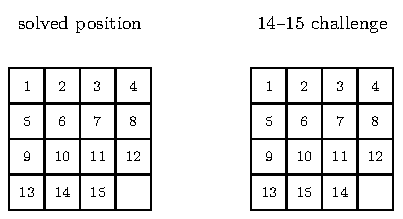
\includegraphics[
                width=0.72\textwidth
            ]{Figures/ExpectedProblems/ReasoningandPuzzleProblems/FifteenPuzzle1415Challenge/ProblemFigure.pdf}
        \end{center}
    \end{expectedproblem}

    \begin{solution}
        Read the tiles row by row from left to right and top to bottom, omitting
        the blank square. Let $I$ be the number of inversions in this resulting
        list, and let $r$ be the row number of the blank square counted from the
        top. We claim that the parity of
        \[
            I+r
        \]
        is invariant under every legal move.

        If the blank square moves horizontally, then the order of the numbered
        tiles in the row-by-row list does not change, so $I$ is unchanged, and
        $r$ is also unchanged. Hence the parity of $I+r$ is unchanged.

        If the blank square moves vertically, then one tile moves up or down by
        one row. In the row-by-row list, that tile passes across exactly three
        other tiles, so the inversion number changes by $3$, and therefore its
        parity changes. At the same time, the blank square moves to an adjacent
        row, so the parity of $r$ also changes. Hence the parity of $I+r$
        remains unchanged in this case as well.

        In the solved position, the inversion number is
        \[
            I=0,
        \]
        and the blank square lies in row $4$, so
        \[
            I+r\equiv0+4\equiv0\pmod2.
        \]
        In the target position, the list differs only by the transposition of
        $14$ and $15$, so
        \[
            I=1,
        \]
        while the blank square is still in row $4$. Thus
        \[
            I+r\equiv1+4\equiv1\pmod2.
        \]
        Since the parity of $I+r$ is invariant, the target position cannot be
        reached from the solved position.

        Therefore the 14--15 challenge is impossible.
    \end{solution}

    \begin{expectedproblem}[Chomp]
        An $m\times n$ rectangular chocolate bar consists of unit-square
        pieces. The lower-left piece is poisoned.

        On each turn, a player chooses one remaining piece and eats that piece
        together with every remaining piece weakly above it and weakly to its
        right. The player who eats the poisoned piece loses.

        Prove that whenever the initial bar contains more than the poisoned
        piece alone, the first player has a winning strategy.
    \end{expectedproblem}

    \begin{solution}
        Since the game is finite and has no draws, one of the two players has a
        winning strategy. Suppose, for contradiction, that the second player
        has one.

        Let the first player eat only the upper-right corner piece. According
        to the supposed winning strategy, the second player must have a
        non-poisoned response; otherwise the second player is forced to eat the
        poisoned piece and loses. Let that response be a remaining piece $C$.
        Eating $C$ also removes the upper-right corner, because that corner
        lies above and to the right of $C$. Hence the position obtained after
        these two moves is exactly the position that would have resulted had
        the first player chosen $C$ on the very first move.

        After the original two-move sequence, this position is losing for the
        player whose turn it is, namely the first player. The first player
        could instead begin by choosing $C$ and hand the identical losing
        position to the second player. This contradicts the assumption that
        the second player has a winning strategy.

        Therefore the first player has a winning strategy. The argument proves
        its existence without identifying the winning first move in general.
    \end{solution}

    \begin{expectedproblem}[Braess's Paradox]
        A total traffic flow of $4000$ units travels from $S$ to $T$ in the
        directed network with routes
        \[
            S\to A\to T
            \qquad\text{and}\qquad
            S\to B\to T.
        \]
        If $x$ denotes the flow on a road, its travel time is given by
        \[
            \begin{array}{c|cccc}
                \text{Road}
                & S\to A & A\to T & S\to B & B\to T\\
                \hline
                \text{Travel time}
                & x/100 & 45 & 45 & x/100
            \end{array}
        \]
        Each driver chooses a route of minimum travel time, taking the total
        road flows as given.

        Determine the equilibrium travel time in the original network. Then a
        new directed road $A\to B$ with travel time $0$ is added. Determine the
        new equilibrium travel time.
    \end{expectedproblem}

    \begin{solution}
        Let $y$ units use the upper route $S\to A\to T$. Then $4000-y$
        units use the lower route, and their travel times are
        \[
            C_U(y)=\frac{y}{100}+45,
            \qquad
            C_L(y)=45+\frac{4000-y}{100}.
        \]
        At equilibrium both routes are used and have equal travel time. Thus
        \[
            \frac{y}{100}+45
            =
            45+\frac{4000-y}{100},
        \]
        so $y=2000$ and
        \[
            C_U=C_L=65.
        \]

        After the road $A\to B$ is added, let $f$, $g$, and $h$ be the flows on
        the routes
        \[
            S\to A\to T,
            \qquad
            S\to B\to T,
            \qquad
            S\to A\to B\to T,
        \]
        respectively. Put
        \[
            x=f+h,
            \qquad
            z=g+h,
        \]
        for the flows on $S\to A$ and $B\to T$. The three route costs are
        \[
            C_U=\frac{x}{100}+45,
            \qquad
            C_L=45+\frac{z}{100},
            \qquad
            C_M=\frac{x+z}{100}.
        \]
        If $f>0$, equilibrium would require $C_U\leq C_M$, which implies
        $z\geq4500$, impossible because the total flow is $4000$. Hence
        $f=0$. Similarly, $g=0$. Therefore
        \[
            h=4000,
            \qquad
            x=z=4000,
        \]
        and every driver uses the new middle route with travel time
        \[
            C_M=40+40=80.
        \]
        Thus adding the zero-time road increases the equilibrium travel time
        from
        \[
            \boxed{65}
            \qquad\text{to}\qquad
            \boxed{80}.
        \]
    \end{solution}

    \begin{expectedproblem}[100 Prisoners and 100 Boxes]
        One hundred prisoners and one hundred boxes are labeled
        $1,2,\ldots,100$. The prisoners' labels are placed in the boxes
        according to a uniformly random permutation.

        The prisoners enter the room one at a time. Each prisoner may open at
        most $50$ boxes and must restore them before leaving. They may agree on
        a strategy beforehand but may not communicate after the process
        begins. They all survive if and only if every prisoner finds their own
        label.

        Find a strategy whose probability of saving all the prisoners is
        greater than $30\%$.
    \end{expectedproblem}

    \begin{solution}
        Regard the contents of the boxes as a permutation $\pi$ of
        $\{1,2,\ldots,100\}$, where box $i$ contains the label $\pi(i)$.
        Prisoner $i$ first opens box $i$. If it contains label $j$, the
        prisoner next opens box $j$, and continues following the labels in
        this way for at most $50$ boxes.

        This procedure follows the cycle of $\pi$ containing $i$. Therefore
        every prisoner finds their own label if and only if every cycle of
        $\pi$ has length at most $50$.

        For $51\leq k\leq100$, the probability that a uniformly random
        permutation contains a $k$-cycle is $1/k$. Moreover, two cycles of
        lengths greater than $50$ cannot occur simultaneously. Hence the
        probability that some cycle is too long is
        \[
            \sum_{k=51}^{100}\frac{1}{k}.
        \]
        The probability that all prisoners survive is therefore
        \[
            1-\sum_{k=51}^{100}\frac{1}{k}
            =
            1-\bigl(H_{100}-H_{50}\bigr)
            \approx
            0.3118278207.
        \]
        Thus the cycle-following strategy saves all the prisoners with
        probability approximately
        \[
            \boxed{31.18\%},
        \]
        which is greater than $30\%$.
    \end{solution}

    \begin{expectedproblem}[St.\ Petersburg Paradox]
        A fair coin is tossed until heads appears for the first time. If the
        first head appears on the $n$th toss, the player receives
        \[
            2^n
        \]
        units of money. Compute the expected payoff. If decisions are based
        only on expected monetary value, determine how large an entry fee it
        would be rational to pay, and explain why the conclusion is regarded
        as paradoxical.
    \end{expectedproblem}

    \begin{solution}
        The probability that the first head appears on the $n$th toss is
        \[
            \left(\frac12\right)^n.
        \]
        Therefore the expected payoff is
        \[
            \Exp[X]
            =
            \sum_{n=1}^{\infty}
            2^n\left(\frac12\right)^n
            =
            \sum_{n=1}^{\infty}1
            =
            \boxed{\infty}.
        \]
        Under the rule of maximizing expected monetary value alone, subtracting
        any finite entry fee still leaves an infinite expected net payoff.
        Thus there is no finite upper bound on the fee that this rule recommends.

        The conclusion conflicts sharply with ordinary judgment. For example,
        the payoff is at most $2$ with probability $1/2$ and at most $4$ with
        probability $3/4$, so most outcomes are small. The infinite expectation
        is driven by extremely rare but extremely large prizes. This mismatch
        shows that expected monetary value alone is not always an adequate
        decision criterion; finite resources, risk, and diminishing marginal
        utility of money can all change a rational valuation.
    \end{solution}

    \expectedproblemsection{Mathematical Intuition Problems}
